\documentclass[10pt,a4paper]{article}
\usepackage[T1]{fontenc}
\usepackage[utf8]{inputenc}
\usepackage{lmodern}
\usepackage[a4paper,left=23mm,right=23mm,top=24mm,bottom=24mm]{geometry}
\usepackage{amsmath,amssymb,amsthm,mathtools}
\usepackage{graphicx,booktabs,array,tabularx,enumitem,xcolor}
\usepackage[font=small,labelfont=bf]{caption}
\usepackage{fancyhdr}
\usepackage{microtype}
\usepackage{placeins}
\usepackage{tikz}
\usepackage[colorlinks=true,linkcolor=blue!45!black,citecolor=blue!45!black,urlcolor=blue!45!black]{hyperref}
\hypersetup{pdfauthor={Ivan Besevic},pdftitle={Complex Geometric Root Calculators}}

\pagestyle{fancy}\fancyhf{}
\fancyhead[L]{\small Complex geometric root calculators}
\fancyhead[R]{\small C5 / Research preprint}
\fancyfoot[C]{\small\thepage}
\renewcommand{\headrulewidth}{0.3pt}
\setlength{\parindent}{0pt}\setlength{\parskip}{5pt plus 1pt}
\setlist{itemsep=2pt,topsep=3pt}
\emergencystretch=3em

\theoremstyle{plain}
\newtheorem{theorem}{Theorem}[section]
\newtheorem{proposition}[theorem]{Proposition}
\newtheorem{lemma}[theorem]{Lemma}
\newtheorem{corollary}[theorem]{Corollary}
\theoremstyle{remark}
\newtheorem{remark}[theorem]{Remark}
\newtheorem{observation}[theorem]{Observation}
\numberwithin{equation}{section}

\newcommand{\C}{\mathbb{C}}\newcommand{\R}{\mathbb{R}}\newcommand{\Hp}{\mathbb{H}}
\newcommand{\D}{\mathbb{D}}
\newcommand{\Tm}{\mathrm{T}}
\DeclareMathOperator{\re}{Re}\DeclareMathOperator{\im}{Im}
\DeclareMathOperator{\Arg}{Arg}\DeclareMathOperator{\Log}{Log}
\DeclareMathOperator{\artanh}{artanh}
\newcommand{\lean}[1]{\texttt{#1}}

\begin{document}

{\small\scshape Constructive geometry \,/\, root iterations \,/\, complex dynamics}

\vspace{6pt}
{\LARGE\bfseries Complex Geometric Root Calculators\par}
\vspace{3pt}
{\large Radical supports of the Pandrosion rectangle for a complex radicand and a real degree:
half-plane theorems with fifth- and ninth-power contraction, and a ninth-order iteration whose basins
are the full sectors\par}
\vspace{8pt}
Ivan Besevic\footnote{Computational assistance: the AI systems ChatGPT (OpenAI) and Claude (Anthropic) were used for derivations, proof development,
numerical experiments, figures and manuscript preparation. The author is responsible for the claims
and their attribution. Section~\ref{sec:evidence} states which results are formal proofs, written
proofs, interval-arithmetic certificates or numerical observations.}
\quad$\cdot$\quad Independent research\\
Version C5 (complex companion of \emph{Geometric Root Calculators}, V28 and V29) \quad$\cdot$\quad
13 November 2026\\
\url{https://github.com/ivan-fr/pandrosion}

\vspace{6pt}\hrule\vspace{8pt}

\textbf{Abstract.}
The rectangle iterations of~\cite{v28,v29} compute $X^{1/p}$ for positive $X$ by ruler and compass; all
of them have the form $u_+=u\,\varphi(X/u^{p})$, where the correction $\varphi$ is fixed by a
\emph{support}. We transpose them to a complex radicand $X\neq0$ and a real degree $p$. The root
then has several determinations ($p$ of them for an integer degree, infinitely many for an
irrational one), there is no order, and Newton's method has fractal basins. For a non-integer
degree the state is the point $u$ together with a determination of its argument. The four supports
that are
symmetric under $t\mapsto1/t$ (the centered arc, which is Halley's method; the decentered arc; the
nested radicals; the three means of~\cite{v29}) behave differently. With principal square roots, each
maps the half-plane $\re(X/u^{p})>0$ into itself, and in the Cayley coordinate
$\eta=(X-u^{p})/(X+u^{p})$
\[
  |\eta_{+}|\le|\eta|^{m},\qquad m=3,\ 5,\ 9,\ 9,
\]
for every real degree $p>2$ and every point of the half-plane. Hence each half-sector
$|\arg(u/r)|<\pi/(2p)$ around a determination $r$ of $X^{1/p}$ lies in the basin of $r$, with an
explicit global rate; for an irrational degree these half-sectors are disjoint strips in the plane
of $\log u$.
For Halley's method convergence on this half-plane is known; for the three radical supports the
statement is new, as are the iterations. The proof reduces, by the Schwarz lemma and a maximum
principle on a strip, to one real inequality on the imaginary axis. For the decentered arc the whole theorem is a Lean theorem, with no hypothesis left open. For the
nested support it is a Lean theorem with a single hypothesis, the boundary inequality, which is
certified by two independent interval-arithmetic computations; for the three means the form is the
same, with a written argument for $p\le4$ and one certificate for $p\ge4$. With the square roots taken as
$\sqrt t\,\sqrt{\,\cdot\,}$, the same method gives, for $p\ge3$, the invariance of the larger sector
$|\arg t|<\frac{5\pi}6$ and the contraction $|\zeta_+|\le|\zeta|^{m}$ in its conformal coordinate
(certificate, not Lean): five sixths of each sector $|\arg(u/r)|<\pi/p$ lie in the basin of $r$.
For these two supports the full sector is not in the basin. For the three-mean support it is: the
whole slit plane $X/u^{p}\notin(-\infty,0]$ is invariant, with
\[
  |\zeta_+|\le|\zeta|^{9},\qquad \zeta=\frac{\sqrt t-1}{\sqrt t+1},\quad t=\frac X{u^{p}},
\]
for every real $p>2$. This is a Lean theorem with no hypothesis left open; the boundary inequality
on the cut has an elementary proof. So the three-mean iteration converges from every $u\neq0$ to
the determination nearest in argument, with order nine, and its basins are exactly the sectors.
Every arithmetic operation of a step is given
as an explicit ruler-and-compass protocol, checked by simulation, with a trace inventory: $12p+57$
traces per step for the arc, $12p+129$ for the nested support and $12p+97$ for the three means. Three by-products: on the positive ray the bound is a global
error estimate for the real iterations of~\cite{v28,v29}; on the circle $|u|=|X|^{1/p}$ the same
iteration is a pure angle $p$-section, so a cube root in $\C$ joins the duplication of the cube and
the trisection of the angle; and the decentered arc is a member of a one-parameter family of conic
supports that also contains Laguerre's and Halley's iterations.

\vspace{4pt}\hrule

\section{Introduction}

For $X>0$ the papers~\cite{v28,v29} study iterations on the Pandrosion rectangle. In the direct state
$u$ (an approximation of $X^{1/p}$) and with the residual $t=X/u^{p}$, every one of them reads
\begin{equation}\label{eq:step}
  u_{+}=u\,\varphi(t),\qquad \varphi(t)=\frac{t+(p-1)\,q(t)}{1+(p-1)\,q(t)},\qquad t=\frac{X}{u^{p}},
\end{equation}
where $q=(\kappa-1)/(p-1)$ is the normalized support slope. The exact support returns
$\varphi_*(t)=t^{1/p}$ in one step. Six approximate supports are studied there: AK (Newton), AD
(Halley), the projective AD (a Pad\'e correction), the decentered arc (order~5), the nested
radicals (order~9) and, in~\cite{v29}, a combination of three means (order~9). On the positive axis
the last three converge globally and monotonically.

\textbf{The complex problem.} Let now $X\in\C\setminus\{0\}$ and let $p>1$ be real. For an integer
$p$ the formula~\eqref{eq:step} makes sense for complex $u\neq0$, and each arithmetic operation it
uses, including a square root, is a finite ruler-and-compass construction on points of the plane.
For a non-integer $p$ the power $u^{p}$ depends on a determination of $\arg u$, and the iteration
is written for a logarithm of $u$ (Section~\ref{sec:setup}). Three things change. The root has
several determinations, so one must say which one is reached. There is no order on $\C$, so monotonicity arguments are gone. And global convergence can
fail badly: for Newton's method the basins of the roots of $z^{3}=1$ are the classical fractal.

\textbf{Results.}
\begin{enumerate}
\item \emph{Structure} (Section~\ref{sec:setup}). The dynamics lives in the residual plane:
  $t_+=t/\varphi(t)^{p}$. The step commutes with the rotation by $2\pi/p$. On the rays through the
  roots it is the real iteration of~\cite{v28}. Rational degrees reduce to integer ones, and
  irrational degrees are approximated with an explicit bound. For a support with
  $q(1/t)=q(t)/t$ (a \emph{reciprocal} support) and real coefficients, the circle $|u|=|X|^{1/p}$
  is invariant: there the iteration only moves the angle.
\item \emph{Conic family} (Proposition~\ref{prop:conic}). The supports $q^{2}=t+a(t-1)^{2}$ contain
  Laguerre's iteration for $z^{p}-X$ ($a=0$), Halley's ($a=\tfrac14$) and the decentered arc
  ($a=\frac{p-2}{12p}$, the only member of order five).
\item \emph{Half-plane theorem} (Theorem~\ref{thm:half}). For AD, the decentered arc, the nested
  radicals and the three means, with principal square roots and any real $p>2$: the half-plane
  $\re t>0$ is mapped into itself and $|\eta_+|\le|\eta|^{m}$ with $m=3,5,9,9$.
\item \emph{Sector theorem} (Theorem~\ref{thm:sector}). For the arc and the nested support with the
  natural branch $q=\sqrt t\,m(w)$ and $p\ge3$: the sector $|\arg t|<\frac{5\pi}6$ is invariant, with
  the same exponents in the coordinate $\zeta=(t^{3/5}-1)/(t^{3/5}+1)$.
\item \emph{Slit-plane theorem} (Theorem~\ref{thm:slit}). For the three means and any real $p>2$:
  the slit plane $t\notin(-\infty,0]$ is invariant and $|\zeta_+|\le|\zeta|^{9}$ with
  $\zeta=(\sqrt t-1)/(\sqrt t+1)$; the cut itself is mapped into the slit plane. This is proved in
  Lean, boundary inequality included.
\item \emph{Consequences} (Section~\ref{sec:cor}). Convergence to the determination nearest in
  argument from every state with $\re(X/u_0^{p})>0$, with an explicit bound, for every real $p>2$;
  for the three means, from every state;
  a starting point constructible by square roots and multiplications that works for every
  $X\neq0$; a global error bound for the real
  iterations; an angle $p$-section theorem on the circle.
\item \emph{Constructions} (Section~\ref{sec:constructions}). Explicit ruler-and-compass protocols
  for the complex product, quotient and square root, a trace inventory of one step for each support,
  and the resulting efficiency indices.
\item \emph{What does not transfer} (Sections~\ref{sec:disk} and~\ref{sec:num}). AK and the
  projective AD do not preserve the half-plane; for AK we recall the known disk statement. Outside
  the sector $|\arg t|<\frac{5\pi}6$ the arc and the nested support still converge on most of each
  sector, but not all of it; we report this numerically and claim nothing more.
\end{enumerate}

\textbf{What is classical, and what we could check.} Convergence regions for Newton's and Halley's
methods for $p$-th roots come from the matrix $p$-th root literature. For the iteration started at
$1$ with radicand $a$ (our $t_0=a$): Iannazzo's region for Newton's method is
$\{\re a>0,\ |a|\le1\}\cup\R^{+}$ and for Halley's method the half-plane $\re a>0$
\cite{iannazzo06,iannazzo08}; Guo proves convergence of Newton's method on the disk $|a-1|\le1$
through a residual relation with nonnegative coefficients~\cite{guo10}; for Halley's method the
analogous residual inequality $|R_{k+1}|<|R_k|^{3}$ on $|R_k|\le1$ is proved
in~\cite{lin10,kouba}. We could not consult the full texts of~\cite{iannazzo08,guo10}; the
statements above are taken from their abstracts and from the restatements
in~\cite{lz08,higham10,kouba}. In particular we do not know by which argument the half-plane
result for Halley's method is proved there, and we do not claim that the inequality
$|\eta_+|\le|\eta|^{3}$ for Halley's method is new. Schr\"oder's family and residual
criteria for complex $p$-th roots are in~\cite{cardoso11a,cardoso11b}; the Pad\'e family
in~\cite{lz09,gklz12}. The degree-two conjugacies go back to Cayley and
Schr\"oder~\cite{cayley,schroder}. The dynamics of Laguerre's iteration on $z^{n}-1$ is studied
in~\cite{curry,belik}. The Schwarz lemma and the Phragm\'en--Lindel\"of principle are standard.
New here are the complex analysis of the three radical supports of~\cite{v28,v29}, the uniform
contractions $|\eta_+|\le|\eta|^{m}$ and $|\zeta_+|\le|\zeta|^{9}$ for them, and the identification
of the conic family. We found the decentered arc, the nested support and the three-mean support in
none of the sources above; our search cannot exclude that they appear elsewhere under another name.
For the three-mean support no separate literature search was made for this version.

\section{The complex rectangle update}\label{sec:setup}

\subsection{Degrees, determinations and the state}

Let $p>1$ be real and write $X=e^{L}$; $L=\Log X$ unless said otherwise. The $p$-th roots of $X$ are
\[
  r_k=e^{\ell_k},\qquad \ell_k=\frac{L+2\pi i k}{p},\qquad k\in\mathbb{Z},
\]
the determinations of $X^{1/p}$ (\lean{determination\_root}). For an integer $p$ there are $p$ of
them. For $p=\mu/\nu$ in lowest terms there are $\mu$, the solutions of $u^{\mu}=X^{\nu}$
(\lean{determination\_rational}). For an irrational $p$ they are pairwise distinct and dense on the
circle $|u|=|X|^{1/p}$.

For an integer $p$ the residual $t=X/u^{p}$ depends only on the point $u$. For any other degree it
depends on a determination of $\arg u$. The state is therefore a logarithm $\ell$ of $u$, that is,
the point $u$ together with its argument not reduced modulo $2\pi$, and one step is
\begin{equation}\label{eq:logstep}
  t=e^{L-p\ell},\qquad \ell_{+}=\ell+\Log\varphi(t),\qquad u=e^{\ell}.
\end{equation}
Then $u_+=u\,\varphi(t)$ (\lean{log\_chart\_state}), and for an integer $p$ this
is~\eqref{eq:step} (\lean{log\_chart\_residual\_nat}). The principal logarithm of $\varphi$ is
well defined wherever it is used below, because $\varphi$ takes no value in $(-\infty,0]$ there.

\subsection{Supports}

Throughout, $h=1/p$, $w=(t-1)^{2}/t=t+1/t-2$, and square roots are principal ($\re\sqrt{\cdot}\ge0$).
The five supports of~\cite{v28} are
\begin{align}
 q_{\mathrm{AK}}&=1, &
 q_{\mathrm{AD}}&=\frac{1+t}{2}, &
 q_{\mathrm{proj}}&=\frac{(4p+1)t+2p-1}{(p+1)t+5p-1},\notag\\
 q_{\mathrm{arc}}&=\sqrt{t+a(t-1)^{2}}, &
 q_{\mathrm{nest}}&=\sqrt{t\Bigl(1+\frac{a\,w}{\sqrt{1+\dfrac{b\,w}{1+c\,w}}}\Bigr)},\label{eq:supports}
\end{align}
with
\[
 a=\frac{1-2h}{12},\qquad b=\frac{(1+h)(3+h)}{30},\qquad
 c=\frac{121-185h-67h^{2}-h^{3}}{840\,(3+h)} .
\]
The sixth support, from~\cite{v29}, combines the arithmetic mean, the geometric mean and a conic
mean of $1$ and $t$:
\begin{equation}\label{eq:qM}
 q_{\mathrm M}=m_0\,(1+t)+g_0\sqrt t-n_0\sqrt{t+d_0(t-1)^{2}},
\end{equation}
\[
 m_0=\frac{(p-2)(47p^{2}+21p+4)}{60p\,(4p^{2}-1)},\quad
 g_0=\frac{16(p+1)(4p^{2}-1)}{15p\,(5p^{2}+4)},\quad
 n_0=\frac{49p\,(p+1)(p^{2}-4)}{10(4p^{2}-1)(5p^{2}+4)},\quad
 d_0=\frac{5p^{2}+4}{84p^{2}},
\]
all positive for $p>2$, with $2m_0+g_0-n_0=1$ and $\frac5{84}<d_0<\frac1{14}$ (these are the
$m,g,n,d$ of~\cite{v29}; here $m$ is already in use). The three terms are the members
$a=\frac14$, $a=0$ and $a=d_0$ of the conic family of Proposition~\ref{prop:conic}.

The exact support is $q_*(t)=\dfrac{t-t^{h}}{(p-1)(t^{h}-1)}=\dfrac1{p-1}\sum_{k=1}^{p-1}t^{k/p}$,
for an integer $p$ the mean of the $p-1$ mean proportionals between $1$ and $t$; with it $\varphi=t^{1/p}$
(\lean{corr\_exact}).

Write $z=\sqrt t$. Since $w+4=(z+1/z)^{2}$, on the half-plane $\re t>0$ (where $|\arg z|<\pi/4$
and, by Section~\ref{sec:half}, principal roots multiply) the four supports AD, arc, nest and
$\mathrm M$ have the form
\begin{equation}\label{eq:recip}
\begin{gathered}
 q(t)=z\,m(w),\qquad m_{\mathrm{AD}}=\tfrac12\sqrt{w+4},\quad m_{\mathrm{arc}}=\sqrt{1+a w},\quad
 m_{\mathrm{nest}}=\sqrt{1+\frac{a w}{\sqrt{1+b w/(1+c w)}}},\\
 m_{\mathrm M}=m_0\sqrt{w+4}+g_0-n_0\sqrt{1+d_0w},
\end{gathered}
\end{equation}
and then
\begin{equation}\label{eq:mobius}
  \varphi=\frac{z+M}{z^{-1}+M},\qquad M=(p-1)\,m(w).
\end{equation}
Because $w$ is invariant under $t\mapsto1/t$, these supports satisfy $q(1/t)=q(t)/t$ and therefore
$\varphi(1/t)=1/\varphi(t)$ (\lean{corr\_reciprocal}). We call them \emph{reciprocal}. The exact
support is reciprocal; AK and the projective AD are not.

\subsection{Ruler and compass in the plane}

\emph{Integer degrees.} Identify points of the plane with complex numbers, with $0$ and $1$ marked.
Sums, products, quotients and principal square roots of constructed points are constructible, so
one step~\eqref{eq:step} with any support in~\eqref{eq:supports} or~\eqref{eq:qM} is a finite
construction.
Section~\ref{sec:constructions} gives explicit protocols and counts their traces.

\emph{Rational degrees.} For $p=\mu/\nu$ we do not iterate with the degree $p$: the determinations
of $X^{1/p}$ are the $\mu$-th roots of $Y=X^{\nu}$, so the integer-degree iteration is applied to
$Y$ with degree $\mu$, as in~\cite[Proposition~4.5]{v28} for positive $X$. This is a finite
construction.

\emph{Irrational degrees.} One step of~\eqref{eq:logstep} needs $e^{-p\ell}$ and is not a finite
construction. The results below hold for the map~\eqref{eq:logstep} as it stands. Constructively,
$p$ is replaced by a rational $p'$, and the principal determination moves by at most
\begin{equation}\label{eq:perturb}
  \bigl|X^{1/p'}-X^{1/p}\bigr|\le2\,\bigl|X^{1/p}\bigr|\,|\Log X|\,\Bigl|\frac1{p'}-\frac1p\Bigr|
  \qquad\text{whenever }|\Log X|\,\Bigl|\frac1{p'}-\frac1p\Bigr|\le1
\end{equation}
(\lean{degree\_perturbation}). We give no complex analogue of the certified enclosures
of~\cite[Section~6]{v28}.

\emph{Other degrees.} Degrees $0<p\le2$ and $p<0$ reduce to $p>2$, determination by determination,
through $X^{1/p}=\bigl(X^{1/(2^{j}p)}\bigr)^{2^{j}}$ and $X^{1/p}=(1/X)^{1/(-p)}$
(\lean{determination\_doubling}, \lean{determination\_neg}), as in~\cite{v28}.

\emph{Two classical problems.} For $p=3$ a complex cube root contains both classical problems: its modulus is a cube root of
$|X|$ and its argument is a third of $\arg X$. Neither is constructible in general, so, as in
Pandrosion's recursive geometry, the constructions below approximate the root; they do not
construct it exactly.

\subsection{Structure}

\begin{proposition}[Residual dynamics, symmetries, invariant curves]\label{prop:structure}
Let $q$ be any support, $p>1$ real and $X=e^{L}\neq0$.
\begin{enumerate}
\item[(i)] The residual evolves autonomously: $t_+=\Tm(t):=t\,e^{-p\Log\varphi(t)}$; for an integer
  $p$, $\Tm(t)=t/\varphi(t)^{p}$.
\item[(ii)] The step commutes with $\ell\mapsto\ell+2\pi i/p$, the rotation of $u$ by the angle
  $2\pi/p$; for an integer $p$ these are the rotations by $p$-th roots of unity.
\item[(iii)] If $\ell=\ell_k+\sigma$ with $\sigma$ real, then $t=e^{-p\sigma}>0$ and
  $\ell_+=\ell_k+\sigma+\ln\varphi(e^{-p\sigma})$: on each ray through a root, the step is the real
  step of~\cite{v28}.
\item[(iv)] If $q$ is reciprocal and $q(\bar t)=\overline{q(t)}$, then $|t|=1$ implies
  $|\varphi(t)|=1$. Hence the circle $|u|=|X|^{1/p}$ is invariant.
\end{enumerate}
\end{proposition}

\begin{proof}
(i) $L-p\ell_+=(L-p\ell)-p\Log\varphi$ (\lean{log\_chart\_residual}; \lean{residual\_update} for
an integer $p$). (ii) The translation changes $L-p\ell$ by $-2\pi i$, so the residual is unchanged
(\lean{step\_rotation} for an integer $p$). (iii) is a substitution. (iv) For $|t|=1$,
$\overline{\varphi(t)}=\varphi(\bar t)=\varphi(1/t)=1/\varphi(t)$ (\lean{corr\_unit\_circle}).
\end{proof}

So the complex problem splits along two curves: on a ray the iteration works on the modulus alone,
and on the circle on the angle alone. The same support and the same order serve both.

\begin{proposition}[Conic family]\label{prop:conic}
Consider the supports $q_a(t)=\sqrt{t+a(t-1)^{2}}$, $0\le a\le\tfrac14$.
\begin{enumerate}
\item[(i)] $a=0$ gives Laguerre's iteration for $f(z)=z^{p}-X$:
 $u-\dfrac{u^{p}-X}{u^{p-1}\bigl(1+(p-1)\sqrt t\bigr)}=u\,\varphi(t)$ with $q=\sqrt t$.
\item[(ii)] $a=\tfrac14$ gives $q=(1+t)/2$, Halley's iteration, whose correction is the M\"obius map
 $\varphi=\dfrac{(p+1)t+p-1}{(p-1)t+p+1}$.
\item[(iii)] $a=\dfrac{p-2}{12p}$ is the decentered arc. It is the only member of order five; the
 others have order three.
\end{enumerate}
\end{proposition}

\begin{proof}
(i) For $f=z^{p}-X$ one has $(p-1)^{2}f'^{2}-p(p-1)ff''=p^{2}(p-1)^{2}u^{2p-2}\,t$, and Laguerre's
formula $u-pf/(f'+\sqrt{\,\cdot\,})$ reduces to the display (\lean{laguerre\_eq\_corr}). (ii) is the
identity $\bigl(\tfrac{1+t}2\bigr)^{2}=t+\tfrac14(t-1)^{2}$ (\lean{halley\_conic},
\lean{halley\_corr}). (iii) With $x=\Log t$ the exact support is $m_*=\dfrac{\sinh((p-1)x/2p)}{(p-1)\sinh(x/2p)}$ and
$w=4\sinh^{2}(x/2)$, so $m_*^{2}=1+\frac{p-2}{12p}\,w+O(w^{2})$. Hence $m_a^{2}=1+aw$ agrees with it to first order in $w$ (contact
order four in $t-1$, hence order five) exactly when $a=\frac{p-2}{12p}$, and to order zero in $w$
(order three) otherwise.
\end{proof}

\begin{proposition}[Degree two]\label{prop:two}
Let $p=2$, $r^{2}=X$ and $\omega=(u-r)/(u+r)$. Then AK gives $\omega_+=\omega^{2}$, AD gives
$\omega_+=\omega^{3}$, the projective AD gives $\omega_+=\omega^{4}$, and the radical supports are
exact in one step. For the three rational supports the basin of $r$ is exactly the half-plane
$\re(u/r)>0$.
\end{proposition}

\begin{proof}
$u_+\mp r=(u\mp r)^{2}/(2u)$ for AK, $(u\mp r)^{3}/(r^{2}+3u^{2})$ for AD and
$(u\mp r)^{4}/(4u(u^{2}+r^{2}))$ for the projective AD (\lean{newton\_two\_sub} to
\lean{proj\_two\_add}). For $a=0$ the support is $\sqrt t$ and $\varphi=\sqrt t$
(\lean{radical\_two\_exact}); at $p=2$ both radical supports reduce to it. The basin statement is
$|\omega|<1$.
\end{proof}

These conjugacies are classical~\cite{cayley,schroder}; they are recorded because they show what
the general statement should look like: a half-plane in a suitable coordinate, and a pure power.

\section{The half-plane theorem}\label{sec:half}

Let $\Hp=\{t:\re t>0\}$ and $\eta(t)=(t-1)/(t+1)$, the Cayley map of $\Hp$ onto the unit disk $\D$
(\lean{cayley\_norm\_lt\_one}). In terms of the state, $\eta=(X-u^{p})/(X+u^{p})$.

\begin{theorem}[Half-plane theorem]\label{thm:half}
Let $p>2$ be real and let $q$ be the support AD, the decentered arc, the nested radicals or the
three means, with principal square roots. Then $\Tm(t)=t\,e^{-p\Log\varphi(t)}$ is holomorphic on
$\Hp$, maps $\Hp$ into $\Hp$, and
\begin{equation}\label{eq:contraction}
  |\eta(\Tm(t))|\le|\eta(t)|^{m}\quad\text{for all }t\in\Hp,\qquad
  m=3\ (\mathrm{AD}),\quad m=5\ (\mathrm{arc}),\quad m=9\ (\mathrm{nest}),\quad m=9\ (\mathrm M).
\end{equation}
For AD the statement also holds for $1<p\le2$.
\end{theorem}

The constant $1$ in~\eqref{eq:contraction} cannot be replaced by a smaller one uniformly: both sides
tend to $1$ as $t\to0$ or $t\to\infty$. Near $t=1$ the bound is far from tight:
$\eta_+\sim2^{m-1}c_m\,p^{1-m}\,\eta^{m}$, where $c_3=\frac{p^{2}-1}{12}$,
$c_5=\frac{(p-2)(p^{2}-1)(3p+1)}{1440}$, $c_9=c_9(p)$ and, for the three means,
$c_{\mathrm M}=\frac{(p^{2}-1)(p^{2}-4)(4p^{2}-1)(17p^{2}+8)}{2^{11}3^{4}5^{2}7^{2}}$ are the
constants of~\cite{v28,v29}; for instance $2^{4}c_5p^{-4}<\frac1{30}$ and
$2^{8}c_{\mathrm M}p^{-8}<\frac1{11000}$.

The proof has three steps: a Schwarz lemma (Lemma~\ref{lem:schwarz}), a boundary criterion for the
invariance of $\Hp$ (Lemma~\ref{lem:boundary}), and the verification of the criterion for each
support. The first two steps are formalized in general (\lean{schwarz\_halfplane},
\lean{strip\_im\_le}, \lean{halfplane\_contraction}); for the decentered arc the third one is too,
and the statement of Theorem~\ref{thm:half} for the arc is the Lean theorem
\lean{arc\_halfplane\_contraction}:
\begin{gather*}
 \forall p>2,\ \forall t,\quad \re t>0\ \Longrightarrow\
 \Bigl|\frac{\Tm(t)-1}{\Tm(t)+1}\Bigr|\le\Bigl|\frac{t-1}{t+1}\Bigr|^{5},\\
 \Tm(t)=t\,e^{-p\Log\varphi(t)},\qquad \varphi=\frac{t+(p-1)q}{1+(p-1)q},\qquad
 q=e^{\frac12\Log(t+a(t-1)^{2})} .
\end{gather*}

\subsection{Schwarz lemma of order \texorpdfstring{$m$}{m}}

\begin{lemma}\label{lem:schwarz}
Let $\Tm:\Hp\to\Hp$ be holomorphic with $\Tm(1)=1$ and $\Tm(t)-1=O((t-1)^{m})$ at $1$. Then
$|\eta(\Tm(t))|\le|\eta(t)|^{m}$ on $\Hp$.
\end{lemma}

\begin{proof}
$F=\eta\circ\Tm\circ\eta^{-1}$ maps $\D$ into $\D$ and vanishes to order $m$ at $0$, so
$F(\zeta)=\zeta^{m}G(\zeta)$ with $G$ holomorphic. On $|\zeta|=\rho<1$, $|G|\le\rho^{-m}$; by the
maximum principle this holds on $|\zeta|\le\rho$, and $\rho\to1$ gives $|G|\le1$
(\lean{schwarz\_order}; with the order stated as $F=O(\zeta^{m})$ and transferred to $\Hp$:
\lean{schwarz\_bigO}, \lean{schwarz\_halfplane}).
\end{proof}

\subsection{Logarithmic chart and boundary criterion}

For $t\in\Hp$ put $x=\Log t$, so $|\im x|<\pi/2$, and $z=e^{x/2}$. For a reciprocal support
$q=z\,m(w)$ define
\begin{equation}\label{eq:Lambda}
  \Lambda(x)=x-p\,\Log\varphi,\qquad \varphi=\frac{z+M}{z^{-1}+M},\qquad \Tm(t)=e^{\Lambda(\Log t)} .
\end{equation}
In the real setting $\Lambda$ is the map $x\mapsto x_+$ of~\cite{v28} ($x=-p\hat e$, with $\hat e$
the logarithmic error), and $\Lambda\equiv0$ for the exact support. The formula is meaningful for
real $p$.

\begin{lemma}[Boundary criterion]\label{lem:boundary}
Let $m$ be continuous on $\{\re w\ge-2\}$, holomorphic in its interior, with $m(\bar w)=\overline{m(w)}$,
$\re m>0$, and $|\Arg m|<\frac\pi4$ on the line $\re w=-2$ (all of which hold if $\re\,(m^{2})>0$).
Then $\varphi$ is holomorphic on $\Hp$ with no value in $(-\infty,0]$,
and $v=\im\Lambda$ is a bounded harmonic function on the strip $|\im x|<\pi/2$, continuous up to the
boundary. On the boundary point $t=iy$, $y>0$, put $\nu=y-1/y$, so that $w=-2+i\nu$, and
$g=\sqrt{w+4}=\sqrt{2+i\nu}$. Then
\begin{equation}\label{eq:N}
 \Arg\varphi(iy)=\arg N,\qquad
 \re N=(p-1)^{2}|m|^{2}+(p-1)\re(\bar m g),\qquad \im N=1+(p-1)\re(mg),
\end{equation}
with $\re N>0$ and $\im N>0$. If moreover
\begin{equation}\label{eq:U}
  \im N\le\tan(\pi/p)\,\re N\qquad\text{for all }\nu\in\R ,
\end{equation}
then $|\im\Lambda|<\pi/2$ on the strip, that is, $\Tm(\Hp)\subset\Hp$.
\end{lemma}

\begin{proof}
For $t\in\Hp$ also $1/t\in\Hp$, so $\re w>-2$, and $|\arg z|<\pi/4$. Since $\re m>0$, the numbers
$z+M$ and $z^{-1}+M$ have positive real parts, which gives the first claim;
$v=\im x-p\Arg\varphi$ is bounded. At $t=iy$, $z=\sqrt y\,e^{i\pi/4}$ and
$N=(z+M)\overline{(z^{-1}+M)}=i+|M|^{2}+z\bar M+M/\bar z$; since $z+1/z=g$, expanding real and
imaginary parts gives~\eqref{eq:N}. On the line both $m$ and $g$ have arguments in
$(-\pi/4,\pi/4)$, so $\re(mg)>0$, $\re(\bar mg)>0$. Thus $0<\Arg\varphi(iy)$, and~\eqref{eq:U} says
$\Arg\varphi(iy)\le\pi/p$. On the upper boundary $v=\pi/2-p\Arg\varphi\in[-\pi/2,\pi/2)$, and by
conjugation symmetry the same holds on the lower boundary with opposite sign. A bounded harmonic
function on a strip with boundary values in $[-\pi/2,\pi/2]$ takes values in that interval
(Phragm\'en--Lindel\"of~\cite{ransford}), and in the open interval by the strong maximum principle,
since $v(0)=0$. In Lean the bound is obtained from Mathlib's Phragm\'en--Lindel\"of theorem for the
strip applied to $e^{\mp i\Lambda}$ (\lean{strip\_im\_le}, \lean{halfplane\_core}); only the closed
inequality $|v|\le\frac\pi2$ is needed for Lemma~\ref{lem:schwarz}, and strictness follows from the
contraction.
\end{proof}

For the exact support $\Arg\varphi_*(iy)=\pi/(2p)$, the midpoint of the allowed interval
$[0,\pi/p]$: the criterion asks that the argument of the correction be wrong by less than
$\pi/(2p)$ along the whole imaginary axis. All reciprocal supports are far from the exact one at
infinity, where $\Arg\varphi(iy)\to0$; the criterion holds there with nothing to spare, and high
local order does not help. Numerically $\sup_y\Arg\varphi(iy)\cdot p/\pi$ is about $0.64$ for AD,
$0.52$ for the arc, $0.52$ for the nested support and $0.503$ for the three means, for all $p$.

A convenient sufficient condition for~\eqref{eq:U} is the pair
\begin{equation}\label{eq:G}
 \im m\cdot\im g\ge0,\qquad
 G(h,\nu):=\pi(1-h)\,|m|^{2}-(1-\pi h)\,\re(mg)-\frac{h}{1-h}\ \ge0 .
\end{equation}
Indeed the first gives $\re(\bar mg)\ge\re(mg)=:R$, so with $\tau=\tan(\pi/p)$,
$\im N-\tau\re N\le1+(1-\tau)(p-1)R-\tau(p-1)^{2}|m|^{2}$, which decreases in $\tau$; at
$\tau=\pi h\le\tan(\pi h)$ it equals $-(p-1)\,G$.

\subsection{Proof of Theorem~\ref{thm:half}}

\emph{Order.} $\Lambda$ is holomorphic near $0$ and real on the real axis, where~\cite{v28} gives
$\Lambda(x)=C\,x^{m}(1+o(1))$ with $C\neq0$ (for the arc and the nested support these limits are
Lean theorems, \lean{ArcOrderFive.order\_five} and \lean{NestedOrderNine.order\_nine}; for the
three means, \lean{ThreeMeanOrderNine.order\_nine} of~\cite{v29}). A
holomorphic function is determined by its restriction to the real axis, so $\Lambda$ vanishes to
order exactly $m$ at $0$ in $\C$, and $\Tm-1$ to order $m$ at $1$ (\lean{bigO\_of\_real\_bound}: an
analytic function that is $O(|x|^{m})$ on the real axis is $O(|z|^{m})$; for the arc,
\lean{arc\_order}). By Lemmas~\ref{lem:schwarz}
and~\ref{lem:boundary} it remains to check the hypotheses on $m$ and~\eqref{eq:U}.

\emph{AD.} Here $\varphi$ is the M\"obius map of Proposition~\ref{prop:conic}(ii), holomorphic on
$\Hp$ for $p>1$, and with $k=\frac{p+1}{p-1}$,
\[
 \Arg\varphi(iy)=\arctan(ky)-\arctan(y/k)\in\bigl(0,\,2\arctan(1/p)\bigr],
\]
the maximum being at $y=1$. Since $\arctan s\le\frac\pi2 s$ on $[0,1]$, $2\arctan(1/p)\le\pi/p$.

\emph{Decentered arc.} $m^{2}=1+aw$ has real part at least $A:=1-2a=\frac{5p+2}{6p}>0$. On the
boundary $m^{2}=A+ia\nu$ and $g^{2}=2+i\nu$, so $\im m$ and $\im g$ both have the sign of $\nu$.
Write $s=|m|^{2}=\sqrt{A^{2}+a^{2}\nu^{2}}\ge A$ and $\gamma=|g|^{2}=\sqrt{4+\nu^{2}}$; then
$a\gamma\le s$ because $2a\le A$. With $R=\re(mg)$ and $R'=\re(\bar mg)\ge R>0$,
\[
 R^{2}\le RR'=(\re m)^{2}(\re g)^{2}-(\im m)^{2}(\im g)^{2}=\tfrac12A\gamma+s\le\frac{s}{2a}
\]
(\lean{arc\_R\_bounds}). If $\tau=\tan(\pi/p)\ge1$, then
$\im N-\tau\re N\le1-(p-1)^{2}A\le0$, because $(p-1)^{2}(5p+2)-6p=(p-2)(5p^{2}+2p-1)\ge0$. If
$\tau<1$, then $p>3$ (indeed $p>4$), and with $k=\sqrt{s/(2a)}\ge\sqrt{A/(2a)}$ it suffices that
$1+(1-\tau)(p-1)k\le\tau(p-1)^{2}\,2a\,k^{2}$. The left side minus the right side decreases in
$\tau$, and $\tau\ge\pi/p\ge3/p$; at $\tau=3/p$ the inequality is
\[
 2p(p-3)(p-1)\,k+2p^{2}\le(p-2)(p-1)^{2}k^{2}\qquad\text{whenever }(p-2)k^{2}\ge5p+2,
\]
which follows from the positivity of two explicit polynomials on $p\ge3$ (\lean{final\_poly}). The
whole chain from the bounds on $R$ to~\eqref{eq:U} is the Lean theorem \lean{arc\_boundary\_core},
and its translation to the complex correction, $0\le\Arg\varphi(iy)\le\pi/p$, is
\lean{arc\_boundary\_arg}.

\emph{Nested radicals.} For $h\in[0,\frac12]$ one has $0<c\le\frac{121}{2520}$ and
$b\le\frac{7}{40}$. Let $\re w\ge-2$. Then $\re(1+cw)\ge1-2c>0.90$, so
$\rho^{2}:=1+\frac{bw}{1+cw}=1+\frac bc\bigl(1-\frac1{1+cw}\bigr)$ has
$\re\rho^{2}\ge1-\frac{2b}{1-2c}>0.61$; hence $\rho=\sqrt{\rho^{2}}$ is holomorphic, $|\rho|>0.78$,
and $\im\rho$ has the sign of $\im w$. Then $\re(w/\rho)=(\re w\,\re\rho+\im w\,\im\rho)/|\rho|^{2}
\ge-2/|\rho|$, so $\re m^{2}=1+a\re(w/\rho)\ge1-2.56\,a\ge0.78$. This gives the hypotheses of
Lemma~\ref{lem:boundary}. On the boundary $\im m^{2}=a(\nu\re\rho+2\im\rho)/|\rho|^{2}$ has the sign
of $\nu$, which is the first condition in~\eqref{eq:G}. For $h\ge1/\pi$ the second one follows from
$G\ge\pi(1-h)\cdot0.78-\frac h{1-h}\ge0.22$. For $0\le h\le1/\pi$ and $\nu\ge0$ (the case $\nu<0$ is
symmetric) $G>0$ is certified by outward-rounded interval arithmetic on the two charts
$\nu\in[0,32]$ and $1/\nu\in[0,\frac1{32}]$ (in the second chart for $G/\nu$, which extends
continuously to $1/\nu=0$), twice and independently: with \texttt{mpmath.iv} (149 and 179 boxes,
smallest certified lower bounds $0.022$ and $2.7\cdot10^{-4}$; \texttt{certify\_halfplane.py}) and
with Arb ball arithmetic and its complex square root (693 and 345 boxes, lower bounds
$2.0\cdot10^{-3}$ and $3.5\cdot10^{-4}$; \texttt{certify\_halfplane\_arb.py}). Both scripts also
re-certify the arc. In Lean, the holomorphy bounds above, the conjugation symmetry and the order
nine in $\C$ are proved, and the statement for the nested support is the theorem
\lean{nested\_halfplane\_contraction}, whose only hypothesis is
$0\le\Arg\varphi(iy)\le\pi/p$ for all $y>0$, the inequality just certified.

\emph{Three means.} Let $\re z\ge0$, $z\ne0$, $\upsilon=z-1/z$, and let $s$ be any square root of
$1+d_0\upsilon^{2}=1+d_0w$. Since $|s|^{2}\le1+d_0|\upsilon|^{2}$ and
$\re s^{2}=1+d_0\bigl((\re\upsilon)^{2}-(\im\upsilon)^{2}\bigr)$,
\[
 (\re s)^{2}=\tfrac12\bigl(|s|^{2}+\re s^{2}\bigr)\le1+d_0(\re\upsilon)^{2},\qquad
 |\re s|\le1+\sqrt{d_0}\,|\re\upsilon|\le1+\sqrt{d_0}\,\re\bigl(z+\tfrac1z\bigr).
\]
Hence, for $m=m_0(z+1/z)+g_0-n_0s$,
\begin{equation}\label{eq:rem}
 \re m\ \ge\ (g_0-n_0)+(m_0-n_0\sqrt{d_0})\,\re\bigl(z+\tfrac1z\bigr)\ \ge\ g_0-n_0=1-2m_0>0,
 \qquad (p-1)(g_0-n_0)>1 .
\end{equation}
Both facts are polynomial: $\sqrt{d_0}\le2d_0+\frac18$,
$m_0-n_0(2d_0+\frac18)=\frac{(p-2)(653p^{4}-441p^{3}+146p^{2}-160)}{240p(4p^{2}-1)(5p^{2}+4)}>0$ and
$(p-1)(g_0-n_0)-1=\frac{(p-2)(73p^{3}+26p^{2}-13p+4)}{30p(4p^{2}-1)}>0$
(\lean{qM\_div\_re}, \lean{cK\_pos}, \lean{gn\_gap}). On the boundary line, for $\nu\ge0$, put
$r=\sqrt{1+d_0w}$, so $r^{2}=1-2d_0+id_0\nu$ and $g^{2}=2+i\nu$. Then
$\im m=\frac\nu2\bigl(\frac{m_0}{\re g}-\frac{n_0d_0}{\re r}\bigr)\ge0$, because
$(\re r)^{2}=\frac12(|r^{2}|+1-2d_0)\ge\frac{d_0}2(|g^{2}|+2)=d_0(\re g)^{2}$ and
$m_0\ge n_0\sqrt{d_0}$; and
\[
 \re m-\im m=\frac{2m_0}{\re g+\im g}+g_0-\frac{n_0(1-2d_0)}{\re r+\im r}\ \ge\ g_0-n_0\sqrt{1-2d_0}>0,
\]
because $(\re r+\im r)^{2}\ge|r|^{2}\ge1-2d_0$. So $0\le\Arg m<\frac\pi4$ on the upper half of the
line: the hypotheses of Lemma~\ref{lem:boundary} and the first condition in~\eqref{eq:G} hold. If
$p\le4$, then $\tan(\pi/p)\ge1$ and
$\im N-\tan(\pi/p)\re N\le\im N-\re N\le1-(p-1)^{2}|m|^{2}\le0$ by~\eqref{eq:rem}. If $p\ge4$, that
is $0\le h\le\frac14$, the inequality $G>0$ of~\eqref{eq:G} is certified with Arb ball arithmetic
(\texttt{certify\_threemean.py}): 141 boxes on $\nu\in[0,36]$ (lower bound $0.030$) and 195 boxes
for $G/\nu$ in the chart $\nu^{-1/2}\in[0,\frac16]$ (lower bound $1.1\cdot10^{-4}$). In Lean the
statement for the three means is \lean{three\_mean\_halfplane\_contraction}, with
$0\le\Arg\varphi(iy)\le\pi/p$ as its only hypothesis. Theorem~\ref{thm:slit} below is a different
statement about the same map, and has no hypothesis left.
\qed

\begin{remark}[Laguerre]\label{rem:laguerre}
For $a=0$ the support is not bounded relative to $t$ at infinity: $\varphi\sim\sqrt t/(p-1)$ and
$\Tm(t)\sim(p-1)^{p}\,t^{\,1-p/2}$, so arguments are multiplied by $1-p/2$ near infinity. The
half-plane can only be preserved there if $|1-p/2|\le1$, that is $p\le4$. This is consistent with
the known behaviour of Laguerre's iteration on $z^{n}-1$: global convergence apart from a two-cycle
for $n=3,4$, and more complicated dynamics for $n\ge5$~\cite{curry,belik}. For $a>0$ the correction
tends to a constant at $0$ and at infinity, which is what makes a half-plane theorem possible.
\end{remark}

\subsection{Beyond the half-plane: a sector theorem}\label{sec:sector}

On $\Hp$ the radical supports are $q=\sqrt t\,m(w)$ with principal roots~\eqref{eq:recip}. Outside
$\Hp$ this product and the principal root of the product differ: $\sqrt{t+a(t-1)^{2}}$ has a cut
along the line $\re t=1-\frac1{2a}$, whereas $\sqrt t\,\sqrt{1+aw}$ does not. We call
$q=\sqrt t\,m(w)$, with each root principal, the \emph{natural branch}. Geometrically the angle of
$t$ is bisected first.

\begin{lemma}\label{lem:natural}
For $p>2$ the natural branches of the arc and of the nested support are holomorphic on the slit
plane $\C\setminus(-\infty,0]$, with $\re m>0$, and~\eqref{eq:mobius} holds there with
$\re(z+M)>0$ and $\re(z^{-1}+M)>0$.
\end{lemma}

\begin{proof}
$w=t+1/t-2$ is real only for $t$ real or $|t|=1$; on the slit plane a real $w$ is positive or lies
in $[-4,0]$. For the arc, $1+aw$ is real only if $w$ is, and then $1+aw\ge1-4a>0$. For the nested
support, $1+cw$ and $\rho^{2}=1+\frac{bw}{1+cw}$ are M\"obius images of $w$ with real coefficients,
so they are real only for real $w$, where $1+cw\ge1-4c>0$ and $\rho^{2}\ge1-\frac{4b}{1-4c}>0.13$;
hence $\rho$ is holomorphic with $\re\rho>0$. If $m^{2}=1+aw/\rho$ were in $(-\infty,0]$, then
$w=-\lambda\rho$ with $\lambda\ge1/a\ge12$, and $\rho$ would be a root of
$f(\rho)=c\lambda\rho^{3}-\rho^{2}-(b+c)\lambda\rho+1$. Since $f(0)>0$ and
$f\bigl(\frac1{(b+c)\lambda}\bigr)<0$, $f$ has three real roots, so $\rho>0$ is real and
$w=-\lambda\rho$ is a negative real, hence $w\in[-4,0)$ and $\rho\le4/\lambda\le\frac13$; but
$\rho\ge\sqrt{0.13}>\frac13$ there. The rest follows from $|\arg z|<\frac\pi2$ and $\re m>0$.
\end{proof}

\begin{theorem}[Sector theorem]\label{thm:sector}
Let $p\ge3$ be real, $\beta=\frac{5\pi}6$, $S=\{t:|\arg t|<\beta\}$, and let $q$ be the natural
branch of the decentered arc or of the nested support. With
$\Lambda(x)=x-p\bigl(\Log(z+M)-\Log(z^{-1}+M)\bigr)$ and $\Tm(t)=e^{\Lambda(\Log t)}$, the map $\Tm$
is holomorphic on $S$, maps $S$ into $S$, and
\[
  |\zeta(\Tm(t))|\le|\zeta(t)|^{m},\qquad \zeta(t)=\frac{t^{3/5}-1}{t^{3/5}+1},\qquad m=5\ (\mathrm{arc}),\quad
  m=9\ (\mathrm{nest}).
\]
\end{theorem}

\begin{proof}
The map $x\mapsto\tanh\frac{3x}{10}$ sends the strip $|\im x|<\beta$ conformally onto $\D$, and
$\zeta(t)=\tanh\frac{3}{10}\Log t$; the Schwarz lemma of order $m$ applies as in
Lemma~\ref{lem:schwarz}, the order at $x=0$ being the same as before since the natural branch
coincides with the principal one near $t=1$. By Lemma~\ref{lem:natural}, $\Lambda$ is holomorphic on
a neighbourhood of the closed strip and $\im\Lambda$ is bounded. As in Lemma~\ref{lem:boundary} it
suffices that $0\le\Arg\varphi\le2\beta/p$ on the ray $t=ye^{i\beta}$, where
$\Arg\varphi=\Arg(z+M)-\Arg(z^{-1}+M)=\arg N$, $N=(z+M)\overline{(z^{-1}+M)}$; the lower ray follows by
conjugation, and $y<1$ from $y>1$ by $\varphi(1/t)=1/\varphi(t)$. With $h=1/p$ and
$K=z\bar m+m/\bar z$,
\[
  h^{2}N=h^{2}e^{i\beta}+(1-h)^{2}|m|^{2}+h(1-h)K .
\]
So $\im K>0$ gives $\arg N\in(0,\pi)$, and $\arg N\le\theta:=2\beta h$ is equivalent to
$\im(Ne^{-i\theta})\le0$, that is, after division by $h$,
\[
 F:=\bigl[h\sin\beta+(1-h)\im K\bigr]\cos\theta-h\cos\beta\,\sin\theta
   -(1-h)^{2}|m|^{2}\,\frac{\sin\theta}{h}-(1-h)\re K\,\sin\theta\ \le0 .
\]
Both $\im K>0$ and $F<0$ are certified with Arb ball arithmetic for $0\le h\le\frac13$ and $y\ge1$
(\texttt{certify\_sector.py}): on $y\in[1,16]$ from the definitions (401 boxes for the arc, 3427
for the nested support), and on $1/y\in[0,\frac1{16}]$ for $F/y$, with $m=z\,n$,
$K=y\bar n+e^{i\beta}n$ and formulas for $y\im n$ free of cancellation (73 and 7927 boxes). The
script first checks that the two sets of formulas agree numerically.
\end{proof}

For an integer $p\ge3$, in terms of the state: if $|\arg(X/u_0^{p})|<\frac{5\pi}6$, that is
$|\arg(u_0/r)|<\frac{5\pi}{6p}$ for the root $r$ nearest in argument, the natural-branch iteration
stays in that sector and converges to $r$, with $|\zeta_n|\le|\zeta_0|^{m^{n}}$. This is five sixths
of the sector $|\arg(u/r)|<\pi/p$, against one half in Corollary~\ref{cor:conv}; the statement for
real $p\ge3$ in the chart~\eqref{eq:logstep} is the same with strips of half-width $\frac{5\pi}{6p}$.

\begin{remark}\label{rem:sector}
Theorem~\ref{thm:sector} is proved with an interval certificate and is not formalized in Lean. The
value $\frac{5\pi}6$ is a choice. Numerically the boundary criterion holds on the rays
$\arg t=\beta$ up to $\beta\approx0.99\pi$ for $p\le4$, $0.95\pi$ for $p=8$ and $0.90\pi$ as
$p\to\infty$, for the arc and the nested support; for AD only up to about $0.74\pi$ for large $p$.
For these supports and $p\ge3$ it fails at $\beta=\pi$: near the zeros of $m$ on the negative axis,
$\varphi\approx t$ and $\Tm(t)\approx t^{1-p}$. In 300-digit arithmetic, on 5600 random points of $S$ and eight degrees
between $3$ and $1000$, the smallest observed $\log|\zeta_+|/\log|\zeta|$ is $5.40$ for the arc and
$9.64$ for the nested support (\texttt{sector\_test.py}).
\end{remark}

\subsection{The three means on the slit plane}\label{sec:slit}

For the three-mean support $m$ does not vanish: by~\eqref{eq:rem}, $\re m_{\mathrm M}\ge g_0-n_0$.
This removes the obstruction of Remark~\ref{rem:sector}. The natural branch is written with three
principal roots. Let $e_1\ge1\ge e_2>0$ be the roots of $d_0Z^{2}-(1-2d_0)Z+d_0$, so that
$e_1e_2=1$ and $t+d_0(t-1)^{2}=d_0(t+e_1)(t+e_2)$, and put
\begin{equation}\label{eq:qMnat}
 q_{\mathrm M}(t)=m_0\,(1+t)+g_0\sqrt t-n_0\sqrt{d_0}\,\sqrt{t+e_1}\,\sqrt{t+e_2} .
\end{equation}
For $t$ off the negative axis, $t+e_j$ is off the negative axis, so $q_{\mathrm M}$ is holomorphic on
the slit plane $S_\pi=\C\setminus(-\infty,0]$. There it equals $\sqrt t\,m_{\mathrm M}(w)$, and on
$\Hp$ it is~\eqref{eq:qM} with principal roots (the three expressions are holomorphic, have the same
square of the radical and agree on the positive axis). On the cut, \eqref{eq:qMnat} with
$\sqrt{-x}=i\sqrt x$ takes the boundary values from the upper half-plane.

\begin{theorem}[Slit-plane theorem]\label{thm:slit}
Let $p>2$ be real, $q=q_{\mathrm M}$ as in~\eqref{eq:qMnat} and $\Tm(t)=t\,e^{-p\Log\varphi(t)}$.
\begin{enumerate}
\item[(i)] $\Tm$ is holomorphic on $S_\pi$, maps $S_\pi$ into itself, and
 \[
   |\zeta(\Tm(t))|\le|\zeta(t)|^{9},\qquad \zeta(t)=\frac{\sqrt t-1}{\sqrt t+1}\qquad(t\in S_\pi).
 \]
\item[(ii)] For $t<0$, $0<\Arg\varphi(t)<\frac{2\pi}p$, so that $\Tm(t)\in S_\pi$.
\end{enumerate}
Consequently $\Tm^{n}(t)\to1$ for every $t\ne0$, with $|\zeta(\Tm^{n}(t))|\le|\zeta(t)|^{9^{n}}$ on
$S_\pi$.
\end{theorem}

Part (i) is the Lean theorem \lean{three\_mean\_slit\_contraction}, stated in the variable
$z=\sqrt t$:
\begin{gather*}
 \forall p>2,\ \forall z,\quad \re z>0\ \Longrightarrow\
 \Bigl|\frac{\mathrm S(z)-1}{\mathrm S(z)+1}\Bigr|\le\Bigl|\frac{z-1}{z+1}\Bigr|^{9},\qquad
 \mathrm S(z)=z\,e^{-\frac p2\Log\tilde\varphi(z)},\\
 \tilde\varphi=\frac{z^{2}+(p-1)\tilde q}{1+(p-1)\tilde q},\qquad
 \tilde q=m_0(1+z^{2})+g_0z-n_0\sqrt{d_0}\,\sqrt{z^{2}+e_1}\,\sqrt{z^{2}+e_2},
\end{gather*}
with $\mathrm S(z)^{2}=\Tm(z^{2})$ (\lean{slit\_residual}) and $\re\mathrm S(z)>0$
(\lean{three\_mean\_slit\_invariant}).

\begin{proof}
\emph{Reduction.} The map $t\mapsto z=\sqrt t$ sends $S_\pi$ onto the right half-plane $\Hp$, and
$\zeta(t)=\eta(z)$. In the variable $z$ the map is $\mathrm S$, the residual map of the correction
$\tilde\varphi$ for the degree $p/2$. By~\eqref{eq:rem}, applied with $s=\tilde R/z$ where
$\tilde R=\sqrt{d_0}\sqrt{z^{2}+e_1}\sqrt{z^{2}+e_2}$, the number $M=(p-1)\tilde q/z$ satisfies
$\re M\ge(p-1)(g_0-n_0)>1$ for $\re z\ge0$, $z\ne0$. So $z+M$ and $z^{-1}+M$ have positive real
parts and $\tilde\varphi=(z+M)/(z^{-1}+M)$ is holomorphic on $\Hp$ with no value in $(-\infty,0]$
(\lean{$\varphi$M\_differentiableAt}, \lean{$\varphi$M\_mem}). It commutes with conjugation on $\Hp$
and on the positive axis it is the real correction of~\cite{v29} (\lean{$\varphi$M\_conj},
\lean{$\varphi$M\_ofReal}); the order nine at $z=1$ follows as in the proof of
Theorem~\ref{thm:half} (\lean{slit\_order}). On the imaginary axis $\tilde\varphi$ has the four
branch points $\pm i\sqrt{e_1}$, $\pm i\sqrt{e_2}$, and the formula for $\tilde q$ is continuous
from the first quadrant only: for $z$ in the closed first quadrant, $z^{2}+e_j$ stays in the closed
upper half-plane, where the principal root is continuous
(\lean{$\varphi$M\_continuousWithinAt}). We therefore apply the argument of
Lemma~\ref{lem:boundary} on the first quadrant, that is to
$\Lambda(\xi)=\xi-\frac p2\Log\tilde\varphi(e^{\xi})$ on the strip $0<\im\xi<\frac\pi2$. On the real
line $\im\Lambda=0$. On the line $\im\xi=\frac\pi2$,
$\im\Lambda=\frac\pi2-\frac p2\Arg\tilde\varphi(i\tau)$, which lies in $[-\frac\pi2,\frac\pi2]$ as
soon as
\begin{equation}\label{eq:cut}
 0\le\Arg\tilde\varphi(i\tau)\le\frac{2\pi}p\qquad\text{for all }\tau>0 .
\end{equation}
Then $\re\mathrm S\ge0$ on the first quadrant by Phragm\'en--Lindel\"of, on the fourth quadrant by
conjugation and on the positive axis because $\mathrm S>0$ there, and Lemma~\ref{lem:schwarz} gives
(i) (\lean{quadrant\_core}, \lean{halfplane\_contraction\_of\_quadrant}).

\emph{The inequality~\eqref{eq:cut}.} Let $z=i\tau$, $\sigma=\tau+1/\tau\ge2$, $c=p-1$, and
$M=A+iB$. Then
\[
 N=(z+M)\,\overline{(z^{-1}+M)}=A^{2}+B^{2}+B\,(\tau-\tfrac1\tau)-1+i\,A\,\sigma,\qquad
 \Arg\tilde\varphi(i\tau)=\arg N .
\]
Replacing $\tau$ by $1/\tau$ changes $B$ into $-B$ and leaves $N$ unchanged, so let $\tau\ge1$ and
$\Delta=\tau-1/\tau=\sqrt{\sigma^{2}-4}$. Since $A>0$, $\im N>0$. The radical is
$\tilde R(i\tau)=i\tau\sqrt{1-d_0\sigma^{2}}$ between the branch points and
$-\tau\sqrt{d_0\sigma^{2}-1}$ above them (\lean{boundary\_R}), which gives two regimes.

(a) $d_0\sigma^{2}\le1$. With $r=\sqrt{1-d_0\sigma^{2}}\in[0,1]$: $A=c\,(g_0-n_0r)$,
$B=c\,m_0\Delta$ and, with $K=c^{2}m_0^{2}+cm_0$,
\[ \re N=A^{2}+K(\sigma^{2}-4)-1>0,\qquad\text{because }A\ge c\,(g_0-n_0)>1 . \]

(b) $d_0\sigma^{2}\ge1$. With $\rho=\sqrt{d_0\sigma^{2}-1}$: $A=c\,g_0$ and
$B=c\,(m_0\Delta-n_0\rho)$. Since $4d_0<1$, $\rho\le\sqrt{d_0}\,\Delta\le(2d_0+\frac18)\Delta$, so
$B\ge c\kappa\Delta\ge0$ with $\kappa=m_0-n_0(2d_0+\frac18)>0$, and
\[ \re N=c^{2}g_0^{2}-1+B^{2}+B\Delta>0 . \]

So $0<\arg N<\frac\pi2$, which proves~\eqref{eq:cut} when $p\le4$. For $p>4$,
$\tan\frac{2\pi}p>\frac{2\pi}p>\frac6p$, and it suffices that
\begin{equation}\label{eq:star}
 p\,\im N\le6\,\re N .
\end{equation}
In regime (a), $\sigma\le1+\frac{\sigma^{2}}4$ and $\sigma^{2}=(1-r^{2})/d_0$, so~\eqref{eq:star}
follows from $F(r)\ge0$ on $[0,1]$, where
\[
 F(r)=6\Bigl[A^{2}+K\Bigl(\frac{1-r^{2}}{d_0}-4\Bigr)-1\Bigr]-pA\Bigl(1+\frac{1-r^{2}}{4d_0}\Bigr)
\]
is a cubic in $r$. In the Bernstein basis,
$150\,p\,(4p^{2}-1)^{2}(5p^{2}+4)^{2}\,F(r)=\sum_{k=0}^{3}\binom3kN_k(p)\,r^{k}(1-r)^{3-k}$, and each
$N_k$ is a polynomial of degree $11$ whose coefficients in powers of $p-4$ are all positive
(\lean{mid\_F}, \lean{mid\_core}). In regime (b), $B^{2}+B\Delta\ge K_2(\sigma^{2}-4)$ with
$K_2=c^{2}\kappa^{2}+c\kappa$, and $\sigma\le\frac{\sigma^{2}}{12}+3$; so~\eqref{eq:star} follows from
\[
 p\,c\,g_0\le72K_2,\qquad 3\,p\,c\,g_0\le6\,(c^{2}g_0^{2}-1)-24K_2 .
\]
The two differences are $\frac{(p^{2}-1)P_{10}(p)}{2400\,D}$ and $\frac{P_{12}(p)}{800\,D}$,
$D=p^{2}(4p^{2}-1)^{2}(5p^{2}+4)^{2}$, with polynomials $P_{10}$, $P_{12}$ whose coefficients in
powers of $p-4$ are all positive (\lean{out\_i}, \lean{out\_ii}, \lean{out\_core}). The polynomials
are listed in the Lean module and recomputed exactly by \texttt{verify\_threemean.py}. This
proves~\eqref{eq:cut} (\lean{boundary\_arg}), hence (i).

\emph{Part (ii).} For $t=-\tau^{2}$ the values of~\eqref{eq:qMnat} are those of $\tilde q(i\tau)$,
and the inequalities above are strict: $\im N>0$, and $\arg N<\frac\pi2\le\frac{2\pi}p$ or
$\tan\arg N\le\frac6p<\tan\frac{2\pi}p$. So $\arg\Tm(t)=\pi-p\Arg\varphi(t)\in(-\pi,\pi)$. The last
assertion follows from (i), since $|\zeta|<1$ on $S_\pi$.
\end{proof}

\begin{remark}\label{rem:slit}
Numerically $\sup_\tau\Arg\tilde\varphi(i\tau)\cdot\frac p{2\pi}$ increases from $0.50$ ($p\to2$) to
$0.568$ ($p\to\infty$): the criterion holds with a margin, where the arc and the nested support
reach the value $1$ before $\beta=\pi$. The criterion also holds numerically on every ray
$\arg t=\beta$, $\frac\pi2\le\beta\le\pi$, so every sector $|\arg t|<\beta$ appears to be invariant;
we prove the two extreme cases, $\beta=\pi$ here and $\beta=\frac\pi2$ in Theorem~\ref{thm:half}.
The iteration is algebraic, not rational: one step takes three square roots. In 300-digit
arithmetic, on 9000 random points of $S_\pi$ and ten degrees between $2.001$ and $1000$, the
smallest observed $\log|\zeta_+|/\log|\zeta|$ is $10.0$ (\texttt{verify\_threemean.py}).
\end{remark}

\section{Consequences}\label{sec:cor}

\begin{corollary}[Convergence to the nearest determination]\label{cor:conv}
Let $p>2$ be real ($p>1$ for AD), $X=e^{L}\neq0$, and let the state $\ell_0$ satisfy
$\re e^{L-p\ell_0}>0$. Let $k$ be the integer with $|\im(L-p\ell_0)+2\pi k|<\frac\pi2$. Then for AD,
the arc, the nested support and the three means, the iteration~\eqref{eq:logstep} satisfies, with
$\eta_n=\eta(e^{L-p\ell_n})$,
\[
 |\eta_n|\le|\eta_0|^{m^{n}},\qquad
 |\ell_n-\ell_k|\le\frac2p\,\artanh\bigl(|\eta_0|^{m^{n}}\bigr),\qquad m=3,\,5,\,9,\,9,
\]
and every $\ell_n$ stays in the strip $|\im\ell-\im\ell_k|<\frac{\pi}{2p}$. Strips around different
determinations are disjoint (\lean{strips\_disjoint}).

For an integer $p$, in terms of the point $u$: if $\re(X/u_0^{p})>0$, the iterates
of~\eqref{eq:step} stay in the half-sector $|\arg(u/r)|<\pi/(2p)$ of the root
$r=u_0\,(X/u_0^{p})^{1/p}$ (principal power) and converge to it, with
$\eta_n=(X-u_n^{p})/(X+u_n^{p})$.
\end{corollary}

\begin{proof}
Let $x_n=L-p\ell_n+2\pi i k$, so $|\im x_0|<\frac\pi2$. By~\eqref{eq:logstep} and
\lean{log\_chart\_conjugacy},
\[ x_{n+1}=x_n-p\Log\varphi(e^{x_n})=\Lambda(x_n), \]
which stays in the strip $|\im x|<\frac\pi2$ by Theorem~\ref{thm:half}. Then $\ell_n=\ell_k-x_n/p$
(\lean{log\_chart\_error}), $x_n=2\artanh\eta_n$ and $|\artanh\eta|\le\artanh|\eta|$.
\end{proof}

\begin{corollary}[Three means: every state converges]\label{cor:all}
Let $p>2$ be real, $X=e^{L}\neq0$, and let $q=q_{\mathrm M}$ as in~\eqref{eq:qMnat}. Let $\ell_0$ be
any state and $k$ an integer with $|\im(L-p\ell_0)+2\pi k|\le\pi$. If the inequality is strict, then
with $x_n=L-p\ell_n+2\pi ik$ and $\zeta_n=\tanh\frac{x_n}4$,
\[
 |\zeta_n|\le|\zeta_0|^{9^{n}},\qquad
 |\ell_n-\ell_k|\le\frac4p\,\artanh\bigl(|\zeta_0|^{9^{n}}\bigr),
\]
and every $\ell_n$ stays in the strip $|\im\ell-\im\ell_k|<\frac\pi p$. If equality holds, $\ell_1$
is in one of the two adjacent open strips and the statement applies from $n=1$.

For an integer $p$: the iteration~\eqref{eq:step} converges from every $u_0\neq0$. The basin of a
root $r$ is the open sector $|\arg(u/r)|<\frac\pi p$ together with one of its two boundary rays,
and these $p$ sets tile the punctured plane. In particular, from $u_0=1$ the iteration converges to
the principal root $e^{\Log X/p}$ for every $X\notin(-\infty,0)$, with
$\zeta_0=(\sqrt X-1)/(\sqrt X+1)$.
\end{corollary}

\begin{proof}
As for Corollary~\ref{cor:conv}, with Theorem~\ref{thm:slit}: $x_{n+1}=\Lambda(x_n)$ stays in the
strip $|\im x|<\pi$, $\zeta(e^{x})=\tanh\frac x4$, and $x_n=4\artanh\zeta_n$. On the boundary lines
part (ii) applies; which of the two adjacent determinations is reached is fixed by the convention
$\sqrt{-x}=i\sqrt x$ in~\eqref{eq:qMnat}.
\end{proof}

So for the three-mean support the picture is complete: the strips $|\im\ell-\im\ell_k|<\frac\pi p$
tile the plane of $\ell$, each one is the basin of its determination, and the rate
$|\zeta_+|\le|\zeta|^{9}$ holds everywhere. No starting procedure is needed
(Corollary~\ref{cor:start} is only required by the other supports).

\begin{figure}[h]
\centering
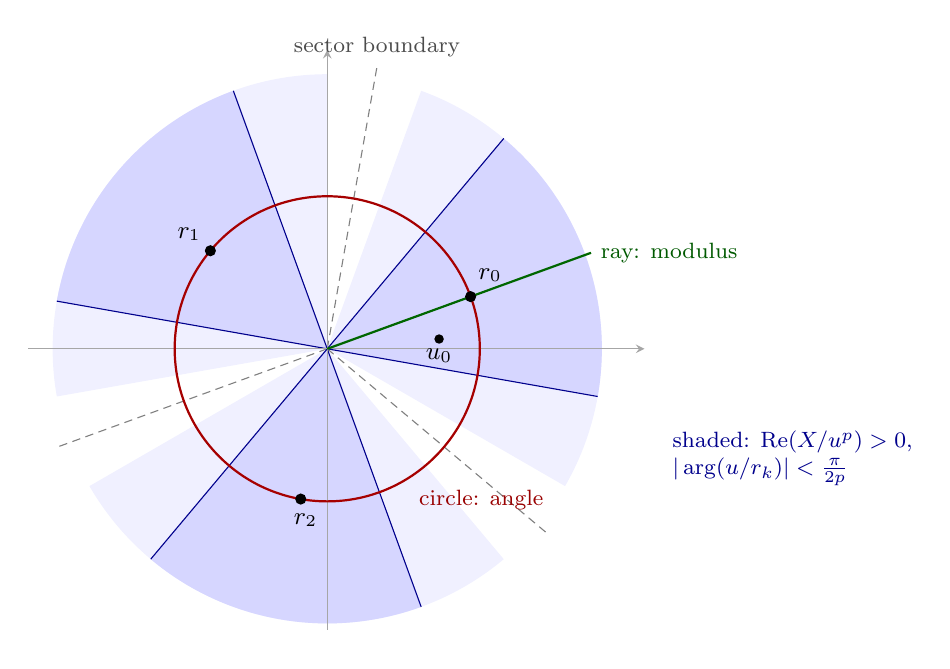
\begin{tikzpicture}[scale=1.55,>=stealth]
  \def\R{1.25}
  \foreach \k in {0,1,2} {
    \fill[blue!6] (0,0) -- ({20+120*\k-50}:2.25) arc ({20+120*\k-50}:{20+120*\k+50}:2.25) -- cycle;
    \fill[blue!16] (0,0) -- ({20+120*\k-30}:2.25) arc ({20+120*\k-30}:{20+120*\k+30}:2.25) -- cycle;
    \draw[densely dashed,gray] (0,0) -- ({80+120*\k}:2.35);
    \draw[blue!55!black,thin] (0,0) -- ({20+120*\k-30}:2.25);
    \draw[blue!55!black,thin] (0,0) -- ({20+120*\k+30}:2.25);
  }
  \draw[->,gray!70] (-2.45,0) -- (2.6,0);
  \draw[->,gray!70] (0,-2.3) -- (0,2.45);
  \draw[red!65!black,thick] (0,0) circle (\R);
  \draw[green!40!black,thick] (0,0) -- (20:2.3);
  \foreach \k/\n in {0/r_0,1/r_1,2/r_2} {
    \fill ({20+120*\k}:\R) circle (1.3pt);
  }
  \node[anchor=south west,font=\small] at (22:\R) {$r_0$};
  \node[anchor=south east,font=\small] at (140:\R) {$r_1$};
  \node[anchor=north,font=\small] at (262:\R+0.03) {$r_2$};
  \fill (5:0.92) circle (1.1pt) node[anchor=north,font=\small] {$u_0$};
  \node[font=\footnotesize,green!35!black,anchor=west] at (20:2.3) {ray: modulus};
  \node[font=\footnotesize,red!60!black,anchor=north west] at (-58:\R+0.02) {circle: angle};
  \node[font=\footnotesize,gray!60!black,anchor=south] at (80:2.35) {sector boundary};
  \node[font=\footnotesize,blue!55!black,align=left,anchor=west] at (2.75,-0.9)
     {shaded: $\re(X/u^{p})>0$,\\ $|\arg(u/r_k)|<\frac{\pi}{2p}$};
\end{tikzpicture}
\caption{The plane of the state for $p=3$. Dark: the three half-sectors, each contained in the
basin of its root with $|\eta_+|\le|\eta|^{m}$ (Corollary~\ref{cor:conv}). Light: the sectors
$|\arg(u/r_k)|<\frac{5\pi}{6p}$ of Theorem~\ref{thm:sector} (natural branch). For the three means the
whole open sector between two dashed rays is the basin of its root (Corollary~\ref{cor:all}). On a
ray through a root
the iteration is the real one of~\cite{v28} (Corollary~\ref{cor:real}); on the circle it only moves
the angle (Corollary~\ref{cor:angle}).}\label{fig:sectors}
\end{figure}

For an integer $p$ the $2p$ rays $\arg(u/r)=\pm\pi/(2p)$ cut out, around each root, a half-sector
contained in its basin (Figure~\ref{fig:sectors}; dashed lines in Figure~\ref{fig:basins}); the $p$
half-sectors cover half of the plane. For an irrational $p$ the determinations are dense on a
circle and a basin in the plane of $u$ has no meaning; in the plane of $\ell$ the certified regions
are the horizontal strips of Figure~\ref{fig:logplane}, which cover half of that plane.

\begin{corollary}[A constructible starting point for every $X$]\label{cor:start}
Let $d/2^{k}$ be a dyadic number with $\bigl|\frac1p-\frac d{2^{k}}\bigr|<\frac1{2p}$, and
$\ell_0=\frac d{2^{k}}\Log X$, that is $u_0=\bigl(X^{1/2^{k}}\bigr)^{d}$: $k$ principal square roots
and $d-1$ multiplications. Then $\re e^{L-p\ell_0}>0$ for every $X\neq0$, and
Corollary~\ref{cor:conv} applies with the principal determination $X^{1/p}=e^{\Log X/p}$. For an
integer $p$ one can take $d=1$ and $\frac23p<2^{k}<2p$. For $p=\mu/\nu$ treated through
$u^{\mu}=X^{\nu}$, the same start works if $\bigl|\frac1p-\frac d{2^{k}}\bigr|<\frac1{2\mu}$.
\end{corollary}

\begin{proof}
$L-p\ell_0=(1-pd/2^{k})\Log X$ has imaginary part of modulus less than $\frac12\pi$. In the rational
case $X^{\nu}/u_0^{\mu}=e^{\mu(1/p-d/2^{k})\Log X}$, with the same conclusion, and the root selected
by the integer-degree statement is $u_0\,e^{(1/p-d/2^{k})\Log X}=e^{\Log X/p}$.
\end{proof}

For $p=3$, $d=1$, $k=2$: two bisections and two mean proportionals give $u_0=X^{1/4}$, and
$\arg(X/u_0^{3})=\frac14\arg X$. The same $u_0$ serves for $p=\pi$.

\begin{corollary}[The ray: global bounds for the real iterations]\label{cor:real}
Let $X>0$, $u>0$ and $p>2$ real. For the decentered arc, the nested support and the three-mean
support of~\cite{v28,v29},
\[
 \frac{|X-u_+^{p}|}{X+u_+^{p}}\le\Bigl(\frac{|X-u^{p}|}{X+u^{p}}\Bigr)^{m},\qquad m=5,\ 9,\ 9,
\]
for \emph{every} positive $u$; for AD the same holds with $m=3$. For the three means, moreover,
\[
 \frac{|\sqrt X-u_+^{p/2}|}{\sqrt X+u_+^{p/2}}\le
 \Bigl(\frac{|\sqrt X-u^{p/2}|}{\sqrt X+u^{p/2}}\Bigr)^{9}.
\]
\end{corollary}

The last inequality, a restriction of \lean{three\_mean\_slit\_contraction} to the positive axis,
is a Lean theorem with no hypothesis. On the positive axis it implies the first one for the three
means, since $\eta=2\zeta/(1+\zeta^{2})$ and $\bigl(\frac{1+\zeta^{2}}2\bigr)^{9}\le\frac{1+\zeta^{18}}2$. These bounds complement~\cite{v28,v29}, which prove global
convergence and the local order but give no quantitative global estimate. With $\theta=\frac{|X-u_0^{p}|}{X+u_0^{p}}<1$ the relative logarithmic
error after $n$ nested steps is at most $\frac2p\artanh(\theta^{9^{n}})$.

\begin{corollary}[The circle: division of an angle by a real number]\label{cor:angle}
Let $p>2$ be real, $|X|=1$, $X=e^{i\alpha}$, and let the state be $\ell=i\beta$. For AD, the arc,
the nested support and the three means the next state is $i\beta_+$, and the angular defect
$\varepsilon=\alpha-p\beta+2\pi k$, if $|\varepsilon|<\frac\pi2$ for some integer $k$, satisfies
\[
 \tan\frac{|\varepsilon_+|}{2}\le\Bigl(\tan\frac{|\varepsilon|}{2}\Bigr)^{m},\qquad m=3,\ 5,\ 9,\ 9 .
\]
For the three means, if only $|\varepsilon|<\pi$:
$\tan\frac{|\varepsilon_+|}{4}\le\bigl(\tan\frac{|\varepsilon|}{4}\bigr)^{9}$.
\end{corollary}

\begin{proof}
Proposition~\ref{prop:structure}(iv), $\eta(e^{i\varepsilon})=i\tan(\varepsilon/2)$ and
$\zeta(e^{i\varepsilon})=i\tan(\varepsilon/4)$.
\end{proof}

So $\beta_n\to(\alpha+2\pi k)/p$. For an integer $p$ this is the $p$-section of an angle. For a
rational $p=\mu/\nu$ it is carried out through $u^{\mu}=X^{\nu}$; for an irrational $p$ it is a
property of the map~\eqref{eq:logstep}, which is not a finite construction.

For the trisection of $\alpha=60^{\circ}$ from $\beta_0=15^{\circ}$ (Corollary~\ref{cor:start}),
$\varepsilon_0=15^{\circ}$ and the bound after one nested step is
$\tan(\varepsilon_1/2)\le\tan(7.5^{\circ})^{9}<1.2\cdot10^{-8}$. The computed defect in $\beta$ is
$1.8\cdot10^{-10}$ degrees after one step and $2.2\cdot10^{-104}$ degrees after two. With the three
means no preparation is needed: from $\beta_0=0$ ($\varepsilon_0=60^{\circ}$) the bound gives a
defect in $\beta$ below $5.5\cdot10^{-4}$ degrees after one step, and the computed defects are
$5.1\cdot10^{-6}$ and $2.4\cdot10^{-65}$ degrees after one and two steps; even from
$\varepsilon_0=170^{\circ}$ the defect is $0.077$, $9.3\cdot10^{-28}$ and $4.8\cdot10^{-261}$
degrees after one, two and three steps. Iterative
approximate trisections are of course old; what is specific here is that the construction is the
cube-root construction itself, restricted to the circle, with a certified global rate.

\section{Ruler-and-compass protocols and inventory}\label{sec:constructions}

Points of the plane are complex numbers; $O=0$, $E=1$ and the real axis are given. A \emph{trace}
is one line through two constructed points ($\mathsf j$) or one circle centred at a constructed
point whose radius is the distance of two constructed points ($\mathsf c$). As in~\cite{v28}, the
parallel to a line through a point is a macro of $2\mathsf j+3\mathsf c$. The unit circle and the
imaginary axis are traced once ($1\mathsf j+3\mathsf c$) and shared by all operations. Real
constants (the coefficients $a,b,c$, $m_0$, $g_0$, $n_0\sqrt{d_0}$, $e_1$, $e_2$ of the supports)
are points of the axis prepared once.

\textbf{Protocols.} For a constructed $Z\neq0$ let $Z_1$ be the point of the unit circle on the ray
$OZ$.
\begin{itemize}
\item \emph{Product $ZW$.} Trace $OZ$ and $OW$. The circle centred $W_1$ of radius $EZ_1$ cuts the
  unit circle at $U$ with $\widehat{W_1U}=\widehat{EZ_1}$: the ray $OU$ has argument
  $\arg Z+\arg W$. The circle $(O,OZ)$ cuts it at $Z_3$. The parallel to $W_1Z_3$ through $W$ cuts
  $OU$ at $P$, and $|OP|=|Z||W|$ by the intercept theorem.
\item \emph{Quotient $Z/W$.} The same with the circle centred $Z_1$ of radius $EW_1$ (argument
  $\arg Z-\arg W$) and the parallel to $WZ_3$ through $W_1$.
\item \emph{Principal square root.} The circles of radius $EZ_1$ centred $E$ and $Z_1$ meet on the
  bisector of $\widehat{EOZ}$. The circle $(O,OZ)$ cuts the negative axis at $Z_4$; the
  perpendicular bisector of $Z_4E$ gives the midpoint $M$; the circle $(M,ME)$ cuts the imaginary
  axis at $H$, with $OH^{2}=|Z|$ (Euclid VI.13); the circle $(O,OH)$ cuts the bisector at $\sqrt Z$.
\item \emph{Sum and difference.} Fourth vertex of a parallelogram, by two arcs.
\item \emph{Multiples.} $nZ$ by $n-1$ compass steps along $OZ$; $\lambda Z$, for a prepared real
  $\lambda>0$, by the parallel to $EZ$ through $\lambda$; the midpoint by a perpendicular bisector.
\end{itemize}

\begin{table}[h]
\centering\small
\begin{tabular}{@{}lccccccc@{}}
\toprule
 & product & quotient & square root & sum, difference & $nZ$ & $\lambda Z$ & midpoint\\
\midrule
traces & $6\mathsf j+5\mathsf c$ & $6\mathsf j+5\mathsf c$ & $3\mathsf j+7\mathsf c$ & $2\mathsf c$
 & $\mathsf j+(n-1)\mathsf c$ & $4\mathsf j+3\mathsf c$ & $2\mathsf j+2\mathsf c$\\
total & 11 & 11 & 10 & 2 & $n$ & 7 & 4\\
\bottomrule
\end{tabular}
\caption{Traces of the elementary protocols (shared setup of four traces not included).}
\label{tab:ops}
\end{table}

\begin{figure}[t]
\centering
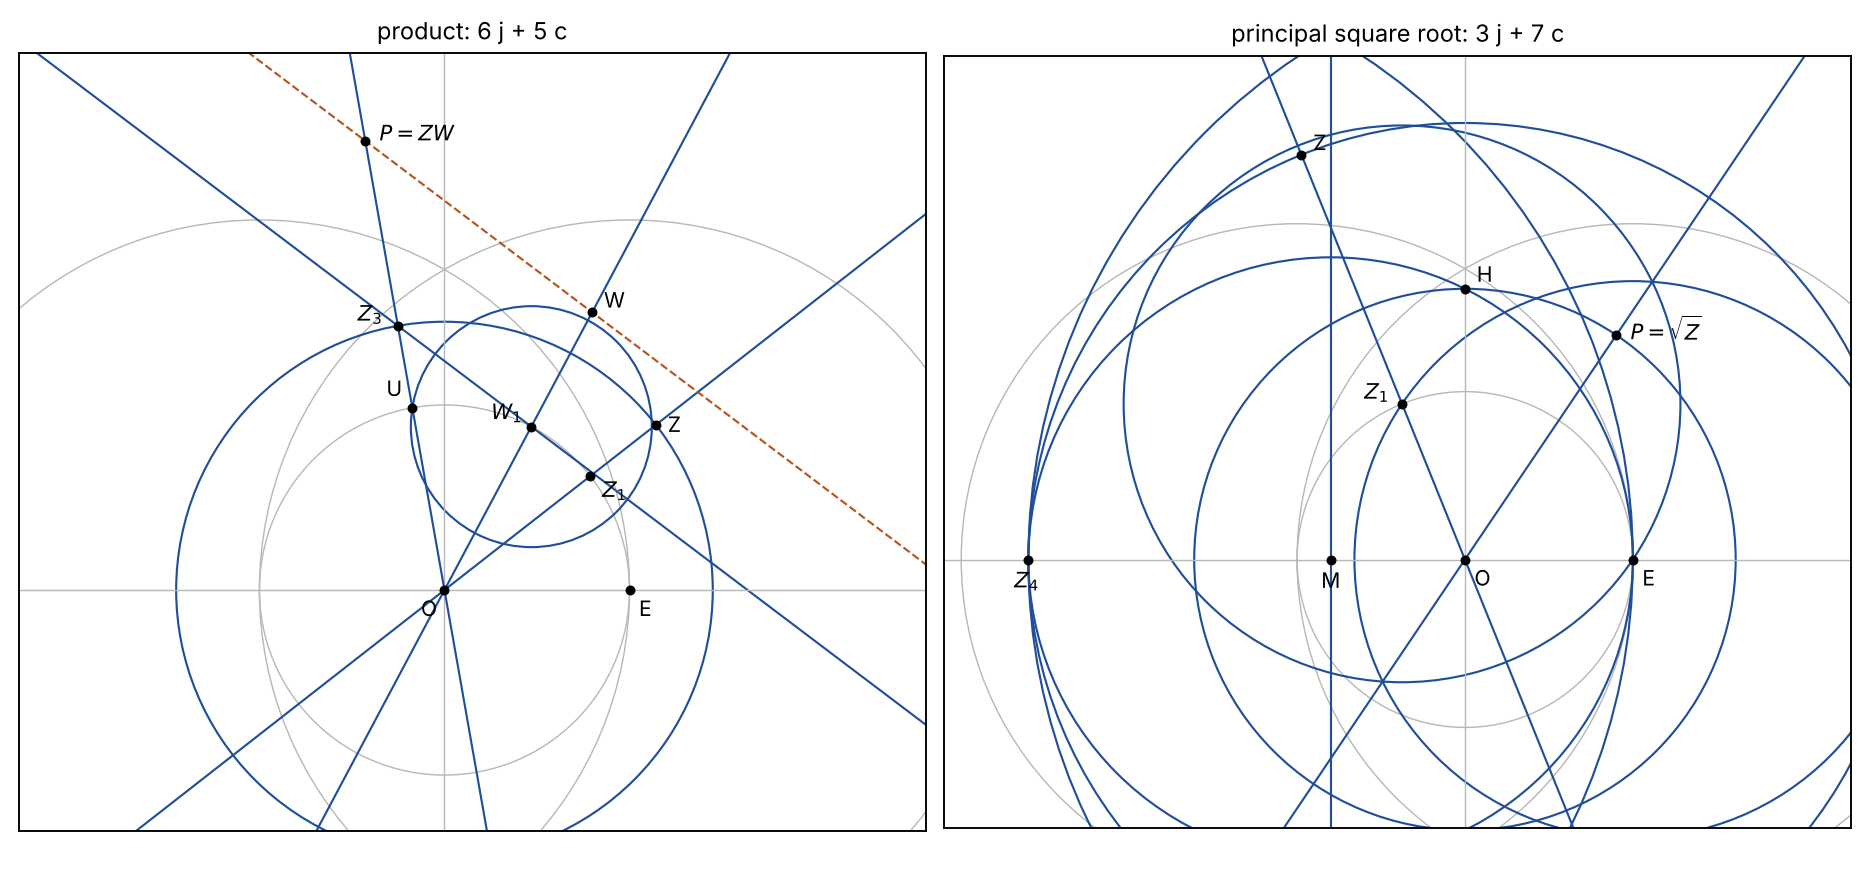
\includegraphics[width=0.92\textwidth]{constructions.png}
\caption{The product and the principal square root, drawn from the traced curves. Grey: shared
setup (unit circle, imaginary axis and its two arcs). Blue: traces of the operation. Dashed: the
parallel, a macro of $2\mathsf j+3\mathsf c$.}\label{fig:constructions}
\end{figure}

The product and quotient protocols need operands off the real axis; a real operand is handled by a
real multiple. This occurs for AK, where $\varphi=(t+p-1)/p$.

\textbf{One step.} A step computes $u^{p}$ by $p-1$ products, the residual $t=X/u^{p}$, the support
$q$, the multiple $(p-1)q$, the two sums $t+(p-1)q$ and $1+(p-1)q$, their quotient $\varphi$ and
the product $u\varphi$: $12p+25$ traces besides $q$ (for AK, where $q=1$ and $\varphi=(t+p-1)/p$ is a sum and a real multiple, $11p+20$ in all). The support costs $4$ traces for AD (a
midpoint), $29$ for the projective AD, $32$ for the arc (a difference, a square, a real multiple, a
sum, a square root), $104$ for the nested support (two products, three quotients, two square
roots, three real multiples and sums) and $72$ for the three means in the form~\eqref{eq:qMnat}
(three square roots, one product, three real multiples, five sums or differences).

\begin{table}[h]
\centering\small
\begin{tabular}{@{}lcccccc@{}}
\toprule
 & AK & AD & projective AD & decentered arc & nested radicals & three means\\
\midrule
order & 2 & 3 & 4 & 5 & 9 & 9\\
traces per step & $11p+20$ & $12p+29$ & $12p+54$ & $12p+57$ & $12p+129$ & $12p+97$\\
\midrule
index, $p=3$ & 0.01308 & 0.01690 & 0.01540 & \textbf{0.01731} & 0.01332 & 0.01652\\
index, $p=5$ & 0.00924 & 0.01234 & 0.01216 & 0.01376 & 0.01163 & \textbf{0.01400}\\
index, $p=8$ & 0.00642 & 0.00879 & 0.00924 & 0.01052 & 0.00977 & \textbf{0.01138}\\
index, $p=12$ & 0.00456 & 0.00635 & 0.00700 & 0.00801 & 0.00805 & \textbf{0.00912}\\
index, $p=16$ & 0.00354 & 0.00497 & 0.00564 & 0.00646 & 0.00684 & \textbf{0.00760}\\
\bottomrule
\end{tabular}
\caption{Traces of one complete step and efficiency index $\ln(\text{order})/\text{traces}$.}
\label{tab:inventory}
\end{table}

With these protocols the decentered arc has the best index for $p=3$ and $p=4$ and the three means
for every $p\ge5$ (the indices cross at $p\approx4.4$). The three means cost $32$ traces less than
the nested support at every degree; without them the arc leads for $3\le p\le11$ and the nested
support for $p\ge12$. The natural branch of Section~\ref{sec:sector}
needs the square root of $t$ and one more product: $12p+89$ traces for the arc and $12p+139$ for the
nested support; the $12p+97$ traces of the three means are already those of the natural
branch~\eqref{eq:qMnat}. The three-arc construction of~\cite{v29}, which costs only two traces more
than the arc on the real rectangle, has no direct analogue here: its lengths become complex
numbers, and each of the three radicals is a full square-root protocol.

\textbf{Checks and limits of the inventory.} Every protocol was executed numerically
(\texttt{geometry.py}): each elementary protocol on 300 random inputs, and complete steps of the
six supports for $p=3,4,5,7$ on 40 random inputs each. Each new point is computed as an
intersection of the traced curves and compared with complex arithmetic, and the trace counts are
compared with the formulas of Table~\ref{tab:inventory}. The protocols are explicit, not optimized:
sharing lines between operations, or computing $u^{p}$ by repeated squaring, would lower the
counts. They are not comparable with the inventories of~\cite{v28,v29}, whose constructions act on the
rectangle with real quantities. On the circle or on a ray (Corollaries~\ref{cor:real}
and~\ref{cor:angle}) the operations degenerate and cheaper protocols apply; we did not count them.

\section{The supports that are not reciprocal}\label{sec:disk}

For AK and the projective AD, $\varphi(t)$ grows linearly at infinity, $\Tm(t)$ behaves like
$t^{1-p}$ there, and no half-plane or sector is invariant when $p\ge3$. A bounded region is needed.

\begin{proposition}[AK on the unit disk; after Guo~\cite{guo10}]\label{prop:newton}
Let $p>1$ be real. For $|1-t|\le1$, $|1-\Tm_{\mathrm{AK}}(t)|\le|1-t|^{2}$.
\end{proposition}

\begin{proof}
With $s=1-t$, $\Tm_{\mathrm{AK}}=(1-s)(1-s/p)^{-p}=(1-s)\sum_{k\ge0}\alpha_ks^{k}$,
$\alpha_k=\frac{p(p+1)\cdots(p+k-1)}{k!\,p^{k}}$. Since $\alpha_k/\alpha_{k-1}=\frac{p+k-1}{kp}\le1$,
with equality for $k=1$, $1-\Tm_{\mathrm{AK}}=\sum_{k\ge2}(\alpha_{k-1}-\alpha_k)s^{k}$ has
nonnegative coefficients of sum $\alpha_1-\lim\alpha_k=1$.
\end{proof}

Hence from $|1-X/u_0^{p}|<1$ Newton's iteration converges quadratically to
$u_0(X/u_0^{p})^{1/p}$; the root selection is as in Corollary~\ref{cor:conv}, since the disk lies in
$\Hp$ (for a non-integer $p$, in the chart~\eqref{eq:logstep}). Residual recurrences of this kind are the standard tool for Newton's and Halley's methods
and for Schr\"oder's family~\cite{guo10,lin10,kouba,cardoso11a}; the argument above is the one
attributed to Guo in~\cite{higham10,kouba}. Convergence regions for the Pad\'e family, to which the
projective AD belongs~\cite[Appendix~A]{v28}, are studied in~\cite{lz09,gklz12}.

\begin{observation}\label{obs:proj}
On random samples of the disk $|1-t|<1$ ($4\cdot10^{5}$ points, $p\in\{3,5,12,50\}$) the projective
AD satisfies $|1-\Tm(t)|\le|1-t|^{4}$, with observed supremum of the ratio between $0.997$ and
$0.999$. We have not proved this inequality.
\end{observation}

\section{Numerical illustrations}\label{sec:num}

\begin{figure}[t]
\centering
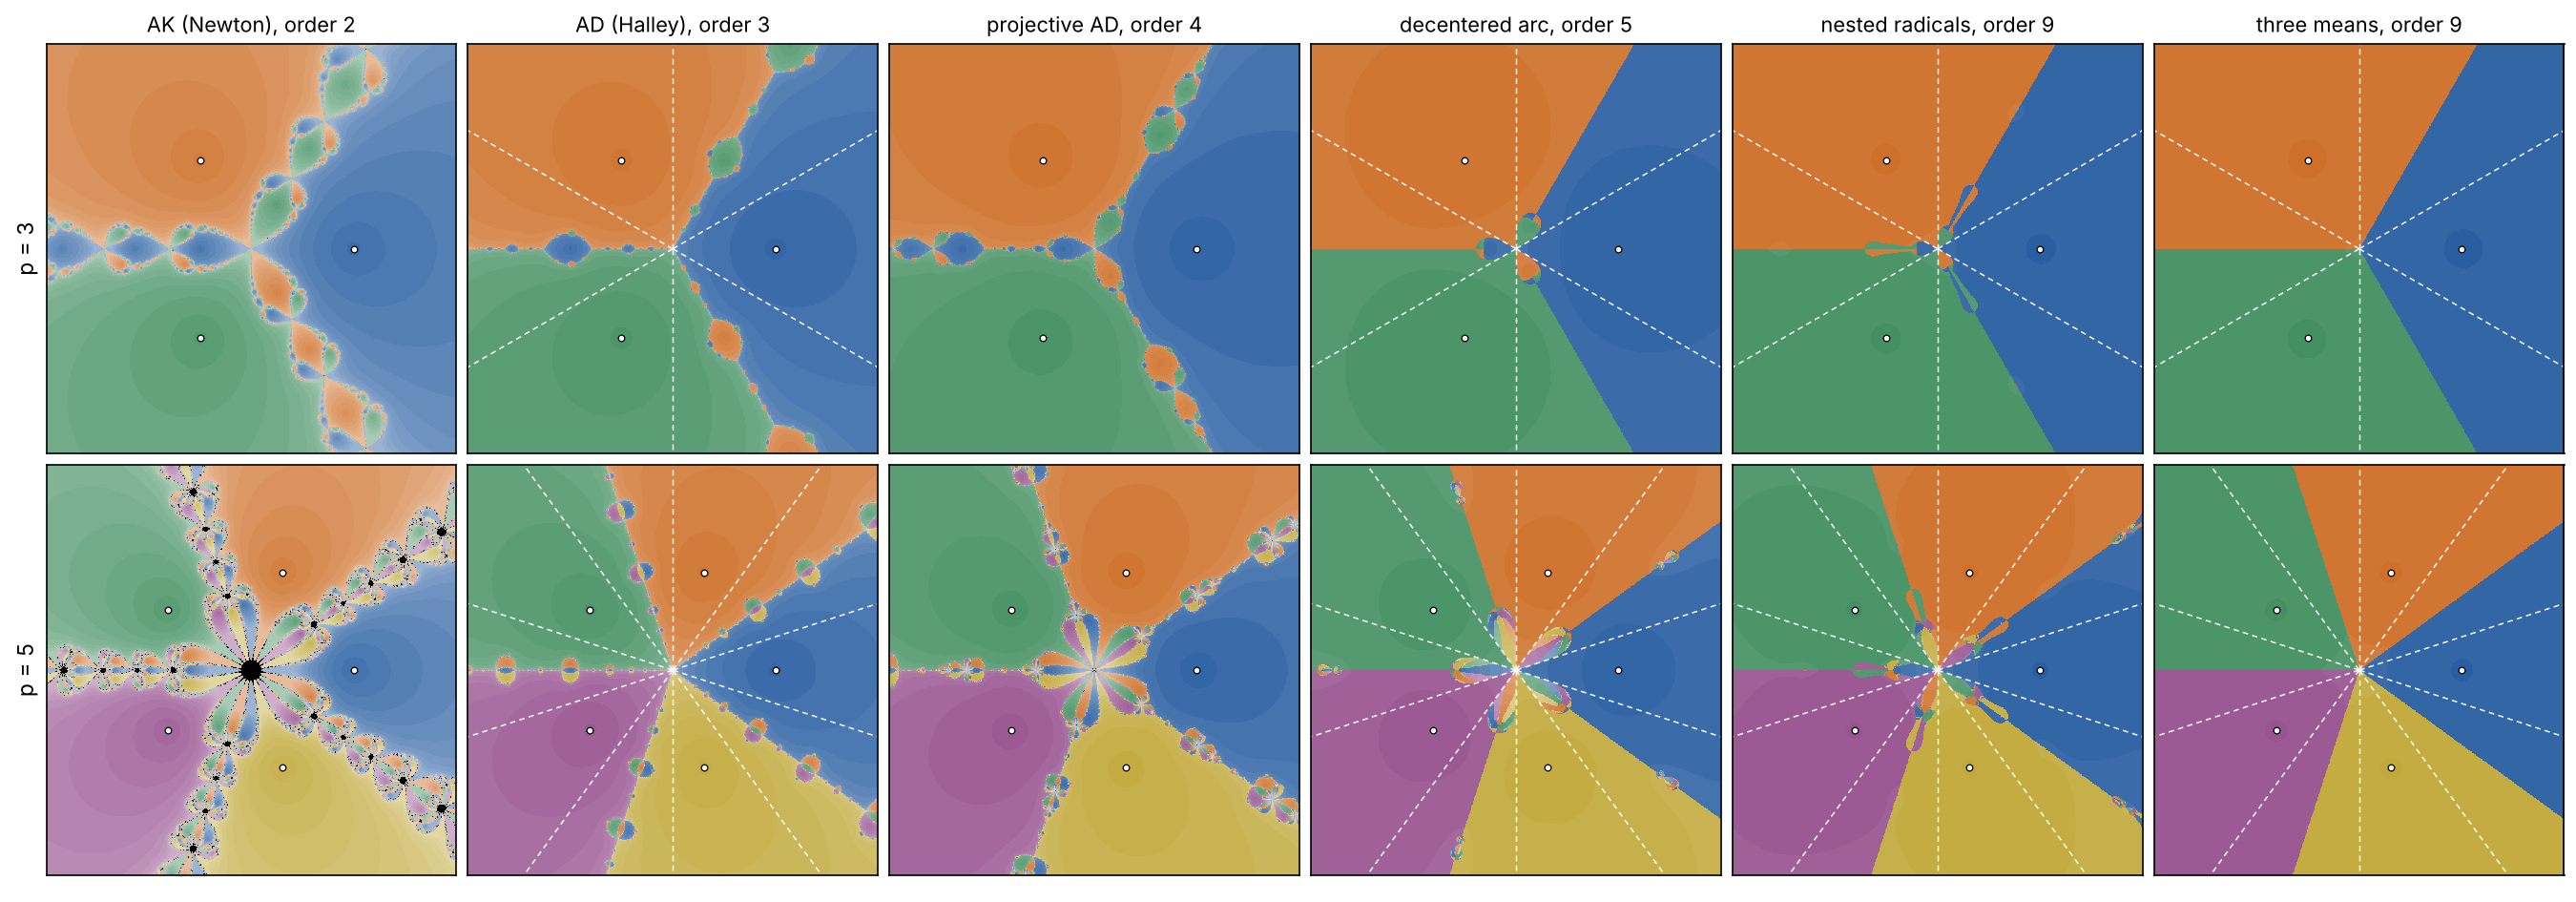
\includegraphics[width=\textwidth]{basins.png}
\caption{Basins of attraction in the plane of the state $u$ for $X=1$, window $[-2,2]^{2}$. Colour:
root reached; darker: more steps; black: no convergence in 40 steps. White dots: the roots. Dashed
(reciprocal supports): boundaries of the half-sectors of Corollary~\ref{cor:conv}. Top row $p=3$,
bottom row $p=5$.}\label{fig:basins}
\end{figure}

Figure~\ref{fig:basins} shows the basins for $X=1$. For AK the picture is the Newton fractal. For
the arc and the nested support the basins look like the sectors $|\arg(u/r)|<\pi/p$ themselves,
except for petals near the origin and thin slivers along the sector boundaries. For the three means
they are the sectors, as Corollary~\ref{cor:all} says. Table~\ref{tab:sector}
gives the share of the window whose points reach the root of their own sector.

\begin{table}[h]
\centering\small
\begin{tabular}{@{}lcccccc@{}}
\toprule
 & AK & AD & projective AD & decentered arc & nested radicals & three means\\
\midrule
$p=3$ & 86.3\% & 96.2\% & 94.6\% & 98.9\% & 98.8\% & 100\%\\
$p=5$ & 77.1\% & 96.0\% & 90.5\% & 97.2\% & 96.8\% & 100\%\\
\bottomrule
\end{tabular}
\caption{Share of the window $[-2,2]^{2}$ ($700^{2}$ points, $X=1$) from which the iteration reaches
the root of the sector containing the starting point.}\label{tab:sector}
\end{table}

\begin{figure}[t]
\centering
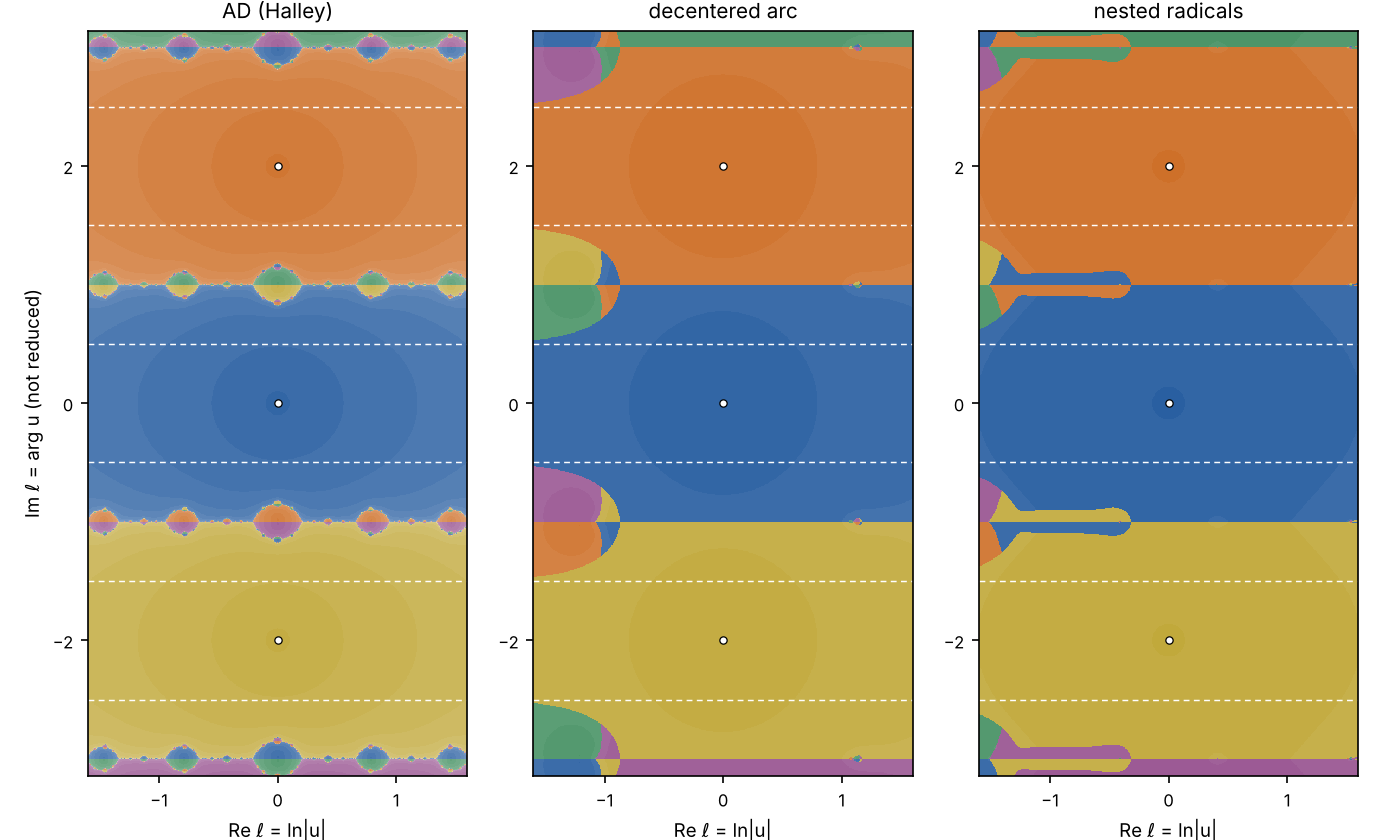
\includegraphics[width=0.78\textwidth]{logplane.png}
\caption{An irrational degree: $p=\pi$, $X=1$, in the plane of the logarithmic state
$\ell=\ln|u|+i\arg u$. Colour: determination reached ($\im\ell_k=2k$); white dots: $\ell_{-1}$,
$\ell_0$, $\ell_1$; dashed: boundaries of the certified strips $|\im\ell-\im\ell_k|<\frac1{2}$ of
Corollary~\ref{cor:conv}.}\label{fig:logplane}
\end{figure}

\textbf{An irrational degree.} Figure~\ref{fig:logplane} shows the same experiment for $p=\pi$ in
the plane of $\ell$. Every sampled state inside the certified strips reaches its determination, as
Corollary~\ref{cor:conv} says. Over the whole window $[-1.6,1.6]\times[-\pi,\pi]$ the share of
states that reach the nearest determination is $94.4\%$ (AD), $91.0\%$ (arc) and $93.1\%$ (nested);
for the three means it is the whole window, by Corollary~\ref{cor:all}.

\textbf{Outside the half-plane.} With principal roots the arc and the nested support are not
holomorphic on the whole slit plane: $q_{\mathrm{arc}}$ has branch points at the two negative roots of $t+a(t-1)^{2}$ and a cut along
the line $\re t=1-\frac{1}{2a}$ (for $p=3$: $\re t=-17$). Near the branch point $t\approx-0.0294$
($p=3$) a fine grid finds starting residuals that converge to a root other than the principal one
(about $2.4\%$ of a box of half-width $0.015$ around it). So the basin of a root is not the full
open sector, and Theorem~\ref{thm:half} does not extend to the slit plane $\C\setminus(-\infty,0]$.
On the coarser grid $|\re t|,|\im t|\le6$ with step $0.02$, which misses that small region, all
but at most $0.005\%$ of the sampled residuals converge to the principal root for the arc
($p=3,4,5,7,12$). For these two supports the largest invariant region is open. For the three means
the question is settled by Theorem~\ref{thm:slit}; Table~\ref{tab:far} follows three starts
$u_0=1$ whose residual is far from the half-plane or close to the cut.

\begin{table}[h]
\centering\small
\begin{tabular}{@{}lccccc@{}}
\toprule
Problem, $u_0=1$ & $\arg t_0$ & $|\zeta_0|$ & $n=1$ & $n=2$ & $n=3$\\
\midrule
$X=-7+i$, $p=5$ & $171.9^{\circ}$ & $0.9543$ & $-2.0\ (-0.18)$ & $-19.6\ (-1.64)$ & $-178.4\ (-14.8)$\\
$X=-1+0.01i$, $p=3$ & $179.4^{\circ}$ & $0.9950$ & $-2.8\ (-0.02)$ & $-26.9\ (-0.18)$ & $-244.4\ (-1.58)$\\
$X=1000i$, $p=7$ & $90^{\circ}$ & $0.9563$ & $-0.6\ (-0.17)$ & $-7.5\ (-1.57)$ & $-69.0\ (-14.2)$\\
\bottomrule
\end{tabular}
\caption{Three means from $u_0=1$: $\log_{10}|\zeta_n|$, and in parentheses the bound
$9^{n}\log_{10}|\zeta_0|$ of Corollary~\ref{cor:all}. In each case the limit is the principal root
$e^{\Log X/p}$.}\label{tab:far}
\end{table}

\begin{table}[h]
\centering\small
\begin{tabular}{@{}llccc@{}}
\toprule
Problem & Support & $n=1$ & $n=2$ & $n=3$\\
\midrule
$X=2+2i$, $p=3$, $|\eta_0|=0.162$ & AD & $-2.9\ (-2.4)$ & $-9.2\ (-7.1)$ & $-28.2\ (-21.3)$\\
 & arc & $-5.9\ (-3.9)$ & $-31.5\ (-19.7)$ & $-159.3\ (-98.7)$\\
 & nested & $-10.5\ (-7.1)$ & $-97.6\ (-63.9)$ & $-881.8\ (-575.3)$\\
 & three means & $-11.5\ (-7.1)$ & $-107.5\ (-63.9)$ & $-971.7\ (-575.3)$\\
\midrule
$X=e^{i\pi/3}$, $p=3$, $|\eta_0|=0.132$ & AD & $-3.2\ (-2.6)$ & $-10.1\ (-7.9)$ & $-30.7\ (-23.8)$\\
 & arc & $-6.4\ (-4.4)$ & $-33.8\ (-22.0)$ & $-171.1\ (-110.1)$\\
 & nested & $-11.3\ (-7.9)$ & $-105.2\ (-71.3)$ & $-950.6\ (-641.9)$\\
 & three means & $-12.3\ (-7.9)$ & $-115.2\ (-71.3)$ & $-1040.7\ (-641.9)$\\
\midrule
$X=-7+i$, $p=5$, $|\eta_0|=0.459$ & AD & $-1.5\ (-1.0)$ & $-5.1\ (-3.0)$ & $-15.7\ (-9.1)$\\
 & arc & $-3.4\ (-1.7)$ & $-18.8\ (-8.5)$ & $-95.9\ (-42.3)$\\
 & nested & $-6.2\ (-3.0)$ & $-58.4\ (-27.4)$ & $-528.7\ (-246.7)$\\
 & three means & $-7.3\ (-3.0)$ & $-69.8\ (-27.4)$ & $-632.2\ (-246.7)$\\
\midrule
$X=2+2i$, $p=\pi$, $|\eta_0|=0.140$ & AD & $-3.1\ (-2.6)$ & $-9.8\ (-7.7)$ & $-29.9\ (-23.1)$\\
\quad($\ell_0=\frac14\Log X$) & arc & $-6.2\ (-4.3)$ & $-32.9\ (-21.4)$ & $-166.3\ (-106.9)$\\
 & nested & $-11.0\ (-7.7)$ & $-102.5\ (-69.3)$ & $-925.5\ (-623.5)$\\
 & three means & $-12.0\ (-7.7)$ & $-112.5\ (-69.3)$ & $-1017.0\ (-623.5)$\\
\midrule
$X=2+2i$, $p=\frac52$, $|\eta_0|=0.081$ & AD & $-3.8\ (-3.3)$ & $-11.8\ (-9.8)$ & $-35.8\ (-29.4)$\\
\quad(via $u^{5}=X^{2}$, $u_0=X^{3/8}$) & arc & $-7.1\ (-5.4)$ & $-37.4\ (-27.2)$ & $-188.5\ (-136.2)$\\
 & nested & $-12.8\ (-9.8)$ & $-118.5\ (-88.2)$ & $-1069.6\ (-794.2)$\\
 & three means & $-14.0\ (-9.8)$ & $-129.8\ (-88.2)$ & $-1172.3\ (-794.2)$\\
\bottomrule
\end{tabular}
\caption{$\log_{10}|\eta_n|$ from the start of Corollary~\ref{cor:start} ($u_0=X^{1/4}$ unless
stated); in parentheses the bound $m^{n}\log_{10}|\eta_0|$ of Corollary~\ref{cor:conv}. Computed
with 1300 digits.}\label{tab:examples}
\end{table}

Table~\ref{tab:examples} follows five problems: three integer degrees, the irrational degree $\pi$
in the chart~\eqref{eq:logstep}, and the rational degree $\frac52$ through the integer degree $5$.
The bound is respected with room to spare, as expected from the small local constants. The three
means gain about one digit per step over the nested support at the first step, in line with the
ratio of the constants $c_{\mathrm M}/c_9$ of~\cite{v29}.

\section{Evidence and reproducibility}\label{sec:evidence}

\textbf{Lean.} Six accompanying modules (Lean~4.33.1, Mathlib~v4.33.1), 198 theorems, no admitted
proof; every theorem depends only on \lean{propext}, \lean{Classical.choice} and \lean{Quot.sound}.
The last module imports the three modules \lean{ThreeMeanGlobal}, \lean{ThreeMeanOrderNine} and
\lean{ThreeMeanWork} of~\cite{v29}, which were recompiled from source in the same environment.
\begin{itemize}
\item \lean{ComplexRoots} (37 theorems). Algebra over $\C$: \lean{residual\_update},
  \lean{step\_rotation}, \lean{corr\_exact}, \lean{corr\_reciprocal}, \lean{corr\_unit\_circle},
  \lean{halley\_conic}, \lean{halley\_corr}, \lean{laguerre\_eq\_corr}, the degree-two identities of
  Proposition~\ref{prop:two}. Real degrees: the four \lean{determination\_*} theorems, the five
  \lean{log\_chart\_*} theorems, \lean{strips\_disjoint}, \lean{degree\_perturbation}. The Schwarz
  lemma \lean{schwarz\_order}, and the real core of the arc case: \lean{arc\_R\_bounds},
  \lean{final\_poly}, \lean{arc\_boundary\_core}.
\item \lean{ComplexHalfPlane} (9 theorems). The general chain: \lean{schwarz\_bigO},
  \lean{schwarz\_halfplane} (Lemma~\ref{lem:schwarz}); \lean{strip\_im\_le} and
  \lean{halfplane\_core} (Lemma~\ref{lem:boundary}, from Mathlib's Phragm\'en--Lindel\"of theorem);
  \lean{bigO\_of\_real\_bound} (from a real order to a complex one); and
  \lean{halfplane\_contraction}, the half-plane theorem for an abstract correction $\varphi$ under
  four hypotheses: holomorphy and values off the negative axis on the closed half-plane, the two
  boundary inequalities, and the order of contact.
\item \lean{ArcHalfPlane} (36 theorems). The four hypotheses for the decentered arc, for every real
  $p>2$: \lean{$\varphi$C\_differentiableAt}, \lean{$\varphi$C\_mem}, \lean{arc\_upper},
  \lean{arc\_lower} (through \lean{arc\_boundary\_arg} and the conjugation symmetry), and
  \lean{arc\_order}, derived from the real theorem \lean{ArcOrderFive.order\_five} of~\cite{v28}.
  Conclusion: \lean{arc\_halfplane\_contraction} and \lean{arc\_halfplane\_invariant}.
\item \lean{NestedHalfPlane} (46 theorems). For the nested support and every real $p>2$: the
  bounds $\re\rho^{2}\ge\frac35$, $\re\rho\ge\frac34$, $\re m^{2}\ge\frac79$ on the closed
  half-plane, holomorphy and values off the negative axis (\lean{$\varphi$N\_differentiableAt},
  \lean{$\varphi$N\_mem}), the conjugation symmetry (\lean{$\varphi$N\_conj}), the identification with
  the real support of~\cite{v28} on the positive axis (\lean{$\varphi$N\_ofReal}), and the order nine
  in $\C$ (\lean{nested\_order}, from \lean{NestedOrderNine.order\_nine} through the general
  \lean{order\_of\_real\_limit}, now stated for every positive degree). Conclusion:
  \lean{nested\_halfplane\_contraction}, with the boundary inequality as its only hypothesis.
\item \lean{ComplexSlitPlane} (4 theorems). The quadrant form of the general chain:
  \lean{strip\_im\_le\_gen} (Phragm\'en--Lindel\"of on a strip $a<\im x<b$), \lean{quadrant\_core},
  \lean{halfplane\_core\_of\_quadrant} and \lean{halfplane\_contraction\_of\_quadrant}: the
  half-plane theorem for a correction that is holomorphic on the open half-plane, continuous on the
  closed first quadrant, symmetric under conjugation and positive on the positive axis, from one
  boundary inequality on the positive imaginary axis.
\item \lean{ThreeMeanSlitPlane} (66 theorems). For the three means and every real $p>2$: the
  principal root with $\sqrt0=0$ and its continuity on the closed upper half-plane; the roots
  $e_1,e_2$ and the factorization of the radicand; \lean{qM\_div\_re} (the bound~\eqref{eq:rem}),
  \lean{$\varphi$M\_mem}, \lean{$\varphi$M\_differentiableAt},
  \lean{$\varphi$M\_continuousWithinAt}, \lean{$\varphi$M\_conj}, \lean{$\varphi$M\_ofReal},
  \lean{slit\_order}; the eight certificate polynomials with their positivity, \lean{mid\_core},
  \lean{out\_core}, \lean{boundary\_R} and \lean{boundary\_arg} (the inequality~\eqref{eq:cut}).
  Conclusions: \lean{three\_mean\_slit\_contraction} and \lean{three\_mean\_slit\_invariant}, with
  no hypothesis; and \lean{three\_mean\_halfplane\_contraction}, with the boundary inequality on
  $\re t=0$ as its only hypothesis.
\end{itemize}
So Theorem~\ref{thm:half} is formally proved for the decentered arc; for the nested support and for
the three means it is formally reduced to the boundary inequality $0\le\Arg\varphi(iy)\le\pi/p$.
Theorem~\ref{thm:slit}(i) is formally proved.

\textbf{Not formalized.} The boundary inequality of the nested support: it rests on the written
argument for its lower half and on the two interval certificates for~\eqref{eq:G}, which rely on
the outward rounding of \texttt{mpmath.iv} and of Arb. The boundary inequality on $\re t=0$ of the
three means: written argument for $p\le4$, one Arb certificate for $p\ge4$. Part (ii) of
Theorem~\ref{thm:slit} (the strict inequalities on the cut; Lean has the closed ones) and the
identification of~\eqref{eq:qMnat} with~\eqref{eq:qM} on $\Hp$, which is checked numerically and
follows from the identity theorem. Corollary~\ref{cor:all} as a statement about iterates.
Theorem~\ref{thm:sector} and
Lemma~\ref{lem:natural} (written proof and the certificate \texttt{certify\_sector.py}). For AD: the
written proof (the order three is classical). Also not formalized: Corollaries~\ref{cor:conv}
to~\ref{cor:angle} as statements about iterates (their algebraic steps are),
Proposition~\ref{prop:newton}, and the geometric protocols of Section~\ref{sec:constructions},
which are checked by simulation.

\textbf{Numerical checks.} \texttt{verify\_complex.py} tests, in 400-digit arithmetic and on random
samples: Theorem~\ref{thm:half} for the three supports and eight degrees between $2.01$ and $1000$
(smallest observed $\log|\eta_+|/\log|\eta|$: $3.29$, $5.89$, $10.69$); the
formulas~\eqref{eq:N}; the invariance of the circle; the constants used for the nested support; the
coefficients in Proposition~\ref{prop:newton}; and the local constants $2^{m-1}c_mp^{1-m}$.
\texttt{verify\_threemean.py} tests, in 300-digit arithmetic: the agreement of the three writings of
the support; Theorem~\ref{thm:slit} (invariance, exponent, the bound~\eqref{eq:rem}); the half-plane
theorem for the three means and its boundary; the two regimes on the cut, with $\re N>0$
and~\eqref{eq:star}; convergence from random residuals of the slit plane and of the cut;
Corollary~\ref{cor:all} for six real degrees; the statement on the circle; the local constants
$2^{8}c_{\mathrm M}p^{-8}$ and $4^{8}c_{\mathrm M}p^{-8}$; and it recomputes exactly, with a
computer-algebra system, every polynomial identity and positivity statement used in the proof
of~\eqref{eq:cut}. \texttt{realdeg.py} tests Corollary~\ref{cor:conv} in the logarithmic chart for the degrees $\pi$,
$\sqrt7$, $\frac52$, $\frac{17}3$, $2.01$ and $40$ (determination reached, strip, bound; smallest
observed ratios $3.02$, $5.04$, $9.07$, and $9.11$ for the three means) and the
bound~\eqref{eq:perturb}. These are tests, not
proofs. \texttt{basins.py}, \texttt{logplane.py}, \texttt{geofig.py}, \texttt{tables.py} and
\texttt{realdeg.py} regenerate the figures and tables; \texttt{geometry.py} runs the protocols of
Section~\ref{sec:constructions}.

\textbf{Changes.} C5 adds the three-mean support of~\cite{v29}: Theorem~\ref{thm:slit},
Corollary~\ref{cor:all}, the fourth case of Theorem~\ref{thm:half}, the Lean modules
\lean{ComplexSlitPlane} and \lean{ThreeMeanSlitPlane}, a sixth protocol and a sixth panel in
Figure~\ref{fig:basins}; Lemma~\ref{lem:boundary} is stated with $\re m>0$ instead of
$\re(m^{2})>0$. C4 added the Lean module \lean{NestedHalfPlane} and the sector theorem
(Section~\ref{sec:sector}). C3 added the Lean modules \lean{ComplexHalfPlane} and \lean{ArcHalfPlane}, the
second certificate, Section~\ref{sec:constructions}, and a more precise account of the literature.
C2 added real degrees (Section~\ref{sec:setup},
Corollaries~\ref{cor:conv} to~\ref{cor:angle}, Figure~\ref{fig:logplane}, eleven Lean theorems)
and corrected one entry of Table~\ref{tab:examples}: the value $-900.7$ printed in C1 for the
nested support at $n=3$ in the trisection problem was the 900-digit precision floor; the value is
$-950.6$.

\section{Scope, limits and open questions}\label{sec:limits}

\begin{itemize}
\item For the arc and the nested support, Theorem~\ref{thm:half} certifies half of each sector and
  Theorem~\ref{thm:sector} five sixths, for the natural branch and $p\ge3$. The full sector is not
  in the basin. The largest invariant sector $|\arg t|<\beta_p$ (numerically between $0.90\pi$ and
  $0.99\pi$) and a description of the true basins are open. For the three means the basins are the
  sectors (Corollary~\ref{cor:all}).
\item Theorem~\ref{thm:slit} is specific to the three-mean support. We do not know which property
  of a reciprocal support is responsible: here it is the lower bound~\eqref{eq:rem} on $\re m$,
  which comes from the two fixed means $A$ and $G$ carrying most of the weight. Whether other
  combinations of conic means, of higher order, share it is open.
\item For an irrational degree a step is not a finite construction. We give the convergence of the
  map and a perturbation bound for rational approximations of the degree, but no certified
  enclosure in $\C$ comparable to the real subdivision of~\cite{v28}, and no bound on the size of
  the integers $\mu,\nu$ needed for a given accuracy.
\item The trace inventory of Section~\ref{sec:constructions} uses explicit but unoptimized
  protocols. Minimal counts, and protocols adapted to the rectangle of~\cite{v28}, are open.
\item Proving Observation~\ref{obs:proj}, for instance by a sign pattern of Taylor coefficients as
  in~\cite{guo10}, is open here.
\item For the nested support, and for the three means on the half-plane, the formal chain stops at
  the boundary inequality on $\re t=0$. A proof of~\eqref{eq:G} without interval arithmetic, or a
  verified interval computation, would complete it. The sector theorem is not formalized at all.
\item The paper~\cite{v29} is a preprint of the same date as this one; its three Lean modules were
  recompiled here, its written proofs were not re-examined.
\item Which members of the conic family, and which higher reciprocal supports, satisfy the boundary
  criterion is a natural question; so is the analogue of Theorem~\ref{thm:half} for matrices with
  spectrum in a half-plane, where the scalar result is the usual first step~\cite{iannazzo08}.
\end{itemize}

\begin{thebibliography}{99}\small
\bibitem{v28} I.~Besevic. \emph{Geometric Root Calculators: a ninth-order nested-radical support and
real-degree enclosures in the Pandrosion rectangle}, V28, 2026.
\url{https://github.com/ivan-fr/pandrosion}.
\bibitem{v29} I.~Besevic. \emph{Geometric Root Calculators: radical supports of orders five and nine
and real-degree enclosures in the Pandrosion rectangle}, V29, 2026.
\bibitem{belik} P.~B\v{e}l\'ik, H.~Kang, A.~Walsh and E.~Winegar. On the dynamics of Laguerre's
iteration method for finding the $n$th roots of unity. \emph{Int. J. Comput. Math.} 2014, Article
ID 321585.
\bibitem{cardoso11a} J.~R.~Cardoso and A.~F.~Loureiro. On the convergence of Schr\"oder iteration
functions for $p$th roots of complex numbers. \emph{Appl. Math. Comput.} 217 (2011).
\bibitem{cardoso11b} J.~R.~Cardoso and A.~F.~Loureiro. Iteration functions for $p$th roots of complex
numbers. \emph{Numer. Algorithms} 57 (2011), 329--356.
\bibitem{cayley} A.~Cayley. The Newton--Fourier imaginary problem. \emph{Amer. J. Math.} 2 (1879), 97.
\bibitem{curry} J.~H.~Curry and S.~L.~Fiedler. On the dynamics of Laguerre's iteration: $Z^{n}-1$.
\emph{Physica D} 30 (1988), 124--134.
\bibitem{gklz12} O.~Gomilko, D.~B.~Karp, M.~Lin and K.~Zi\k{e}tak. Regions of convergence of a
Pad\'e family of iterations for the matrix sector function and the matrix $p$th root.
\emph{J. Comput. Appl. Math.} 236 (2012).
\bibitem{guo10} C.-H.~Guo. On Newton's method and Halley's method for the principal $p$th root of a
matrix. \emph{Linear Algebra Appl.} 432 (2010), 1905--1922.
\bibitem{higham10} N.~J.~Higham and A.~H.~Al-Mohy. Computing matrix functions. \emph{Acta Numerica}
19 (2010), 159--208.
\bibitem{iannazzo06} B.~Iannazzo. On the Newton method for the matrix $p$th root. \emph{SIAM J.
Matrix Anal. Appl.} 28 (2006), 503--523.
\bibitem{iannazzo08} B.~Iannazzo. A family of rational iterations and its application to the
computation of the matrix $p$th root. \emph{SIAM J. Matrix Anal. Appl.} 30 (2008), 1445--1462.
\bibitem{kouba} O.~Kouba. A note on the positivity of the coefficients of some power series
expansions. arXiv:1104.0470, 2011.
\bibitem{lz08} B.~Laszkiewicz and K.~Zi\k{e}tak. Algorithms for the matrix sector function.
\emph{Electron. Trans. Numer. Anal.} 31 (2008), 358--383.
\bibitem{lz09} B.~Laszkiewicz and K.~Zi\k{e}tak. A Pad\'e family of iterations for the matrix sector
function and the matrix $p$th root. \emph{Numer. Linear Algebra Appl.} 16 (2009).
\bibitem{lin10} M.~Lin. A residual recurrence for Halley's method for the matrix $p$th root.
\emph{Linear Algebra Appl.} 432 (2010), 2928--2930.
\bibitem{ransford} T.~Ransford. \emph{Potential Theory in the Complex Plane}. Cambridge University
Press, 1995.
\bibitem{schroder} E.~Schr\"oder. Ueber unendlich viele Algorithmen zur Aufl\"osung der Gleichungen.
\emph{Math. Ann.} 2 (1870), 317--365.
\end{thebibliography}

\end{document}
